\documentclass{scrbook}
\usepackage{graphicx} % Required for inserting images
\usepackage{tabularx} % Required for fixed width tables
\usepackage{scrlayer-scrpage} % Required for the subtitles
\usepackage{url} % Required for the URLs
\usepackage{hyperref} % Required for the URLs
\usepackage{listings} % Required for the code snippets
\usepackage{mathtools} % Required for the system of equations
\usepackage{enumitem} % Required for list styling

\usepackage{fontspec}
\setmonofont{DejaVu Sans Mono} % Overleaf has this font pre-installed

% Put the caption of the snippets at the bottom
\lstset{
	captionpos=b,
	basicstyle=\ttfamily\small,
	columns=fullflexible,
	keepspaces=true
}


\title{HTTP: HyperText Transfer Protocol}
\subtitle{Ambient intelligence course (A.Y. 2025/2026)\\Topic taught by Proff. Michele Ruta \& Floriano Scioscia}
\author{Gabriele Colapinto}
\date{\today}

\begin{document}
	
	\maketitle
	\thispagestyle{empty}
	
	{\Large\textbf{License}} \\
	{Notes from Ambient intelligence (A.Y. 2025/2026) by Gabriele Colapinto. 
		Course taught by professors Michele Ruta, Floriano Scioscia, Arnaldo Tomasino, Davide Loconte — 
		Licensed under CC BY-NC 4.0.\\
		\url{https://creativecommons.org/licenses/by-nc/4.0/}}
	
	\vspace*{\fill}
	\rule{\textwidth}{0.2pt}
	\small{© 2025 Gabriele Colapinto \\
		Released under the \href{https://creativecommons.org/licenses/by-nc/4.0/}{Creative Commons Attribution–NonCommercial 4.0 International License}}
	
	\clearpage
	
	\tableofcontents

\chapter{HTTP Fundamentals and Architectural Entities}

\section{Purpose and Scope of HTTP}

The HyperText Transfer Protocol, commonly abbreviated as \texttt{HTTP}, is an application-layer protocol for collaborative and distributed hypermedia information systems. Its original purpose was the exchange of hypertext documents between a requesting application and a serving application, but its role has progressively widened. In current Web architectures, HTTP is used not only for HTML pages, but also for images, binary files, executable objects, structured data, service interfaces, and distributed application resources.\\

This broad applicability is possible because HTTP does not impose a single representation format on the resources it transfers. The protocol defines how a client and a server exchange requests and responses, while the concrete representation of the resource is described separately through metadata, especially headers. As a consequence, the same application-level protocol can support many kinds of contents and can be used in scenarios that are far from the original transfer of static hypertext.\\

HTTP is characterized by two fundamental properties:
\begin{itemize}
    \item it is \textbf{generic}, because the protocol is not bound to a specific data format or a specific resource type;
    \item it is \textbf{stateless}, because each request is processed independently unless additional mechanisms are used to reconstruct a context.
\end{itemize}

Several mechanisms developed around these two properties are central to the protocol: negotiation of data formats, caching policies, and user authentication procedures. These mechanisms allow HTTP to remain simple at its core while supporting heterogeneous clients, heterogeneous resources, and restricted areas of Web applications.

\section{HTTP in the TCP/IP Stack}

\begin{figure}
	\centering
	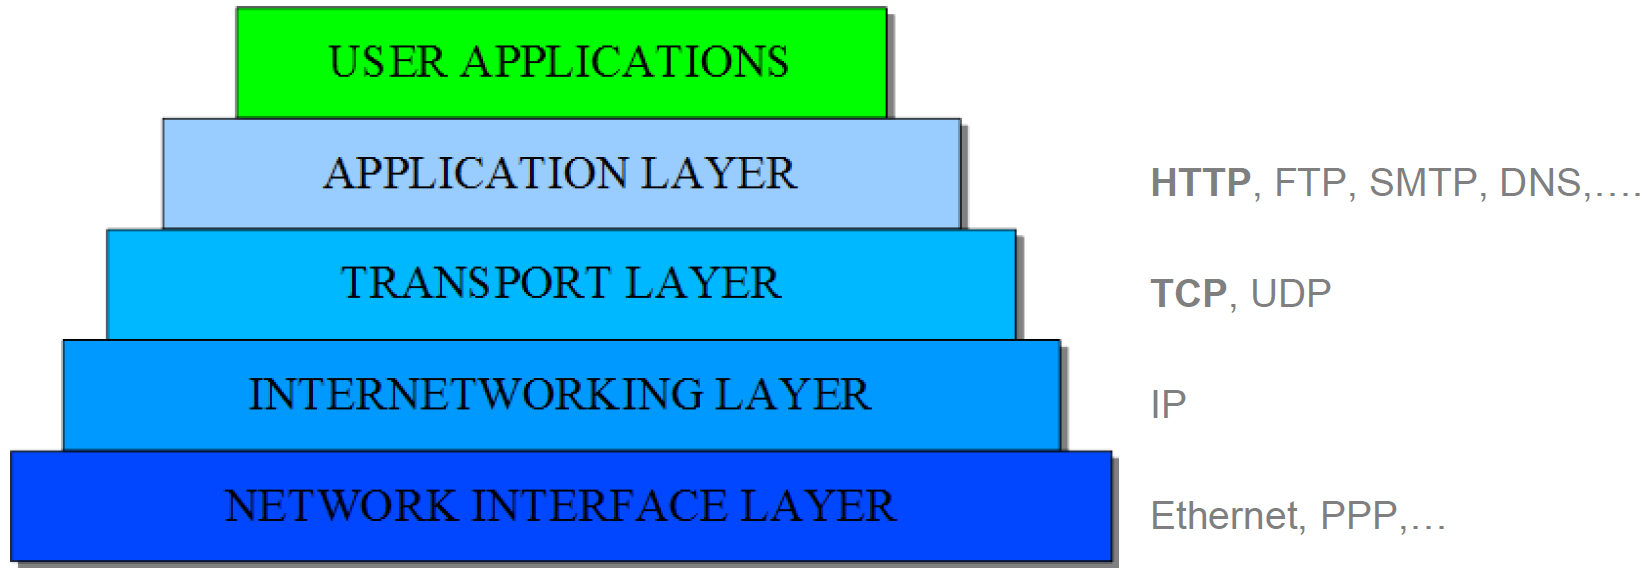
\includegraphics[width=0.5\linewidth]{Images/Protocol_stack.png}
	\caption{TCP/IP stack with protocols}
	\label{fig:protocol_stack}
\end{figure}

\begin{figure}
	\centering
	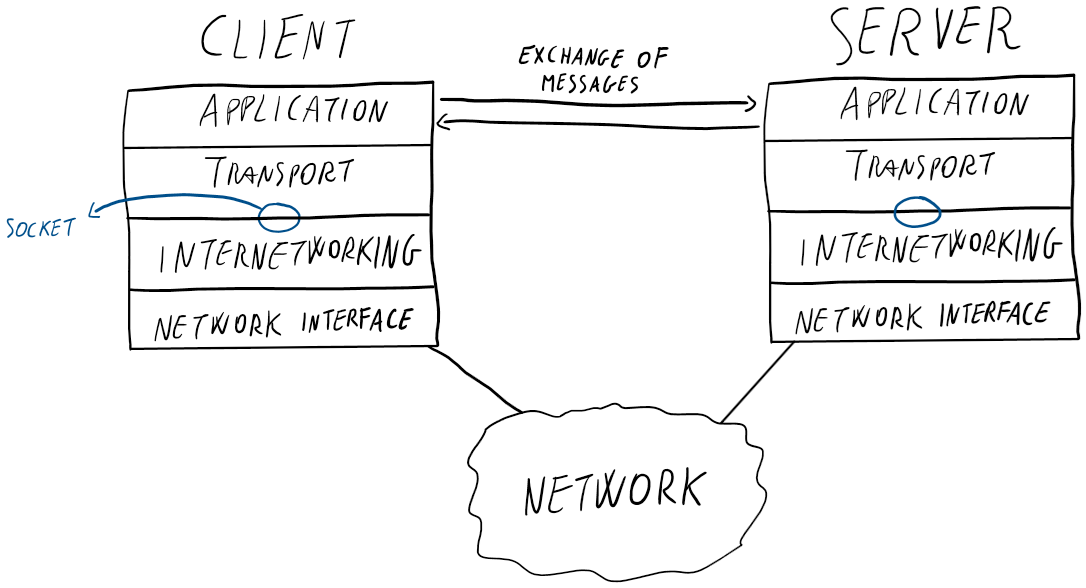
\includegraphics[width=0.5\linewidth]{Images/Exchange_of_messages.png}
	\caption{Exchange of messages at the application protocol}
	\label{fig:exchange_of_messages}
\end{figure}

HTTP operates at the application layer (see figure \ref{fig:protocol_stack}). It relies on the lower layers of the TCP/IP stack to transmit its protocol data units across the network. In a typical stack, HTTP is placed together with other application protocols such as \texttt{FTP}, \texttt{SMTP}, and \texttt{DNS}; below it, transport services are provided by protocols such as \texttt{TCP} or \texttt{UDP}; below transport, \texttt{IP} provides network addressing and routing; and link-layer technologies such as Ethernet or \texttt{PPP} provide access to the physical medium (see figure \ref{fig:exchange_of_messages}).\\

In the standard configuration, HTTP uses \texttt{TCP} as its transport protocol. The default TCP port for ordinary HTTP service is port \texttt{80}. Port \texttt{8080} is also commonly used as an alternative, especially for development servers, proxies, test deployments, or services that should not bind to the privileged default port.\\

From the point of view of HTTP semantics, the lower layers are abstracted by the communication endpoint offered to the application. The protocol can therefore be studied as a logical interaction between two application-level entities: a client-side entity that constructs an HTTP request and a server-side entity that interprets the request and produces an HTTP response. The actual transmission involves encapsulation through the transport, network, and link layers, followed by decapsulation at the destination, but the HTTP message delivered to the server is the application-layer message generated by the client.\\

This abstraction is important because it separates application concerns from network-transfer concerns. HTTP specifies the request, the response, the metadata, the resource identification, and the behavior expected from the communicating applications. It does not define routing, medium access, or packet forwarding.

\section{Client--Server and Request--Response Operation}

\begin{figure}
	\centering
	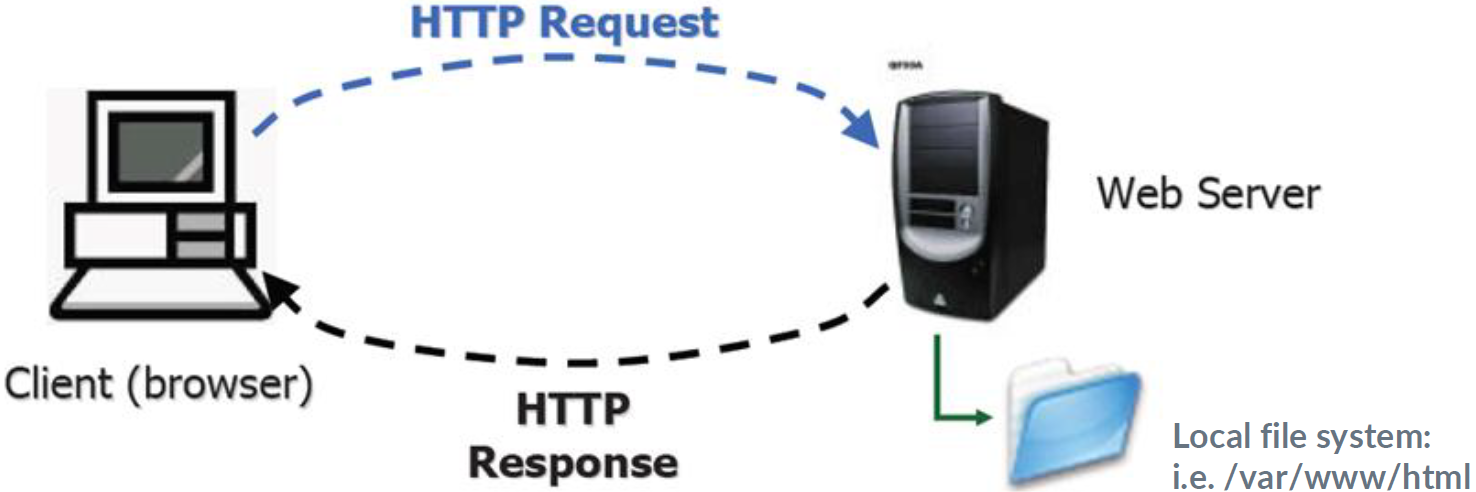
\includegraphics[width=0.5\linewidth]{Images/Client_server_model.png}
	\caption{HTTP client server model}
	\label{fig:client_server_model}
\end{figure}

HTTP follows a client--server model (see figure \ref{fig:client_server_model}). The client initiates communication by opening an HTTP connection and sending a request. The server accepts the connection, interprets the request, and returns a response. The server has a passive role with respect to the beginning of the exchange: it does not start the interaction, but waits for requests and reacts to them.\\

The protocol is also a request--response protocol. An HTTP interaction is structured as a sequence of requests and corresponding responses. A request identifies the action desired by the client and the resource to which that action applies. A response reports the outcome of the request and, when appropriate, carries a representation of the requested resource or metadata about it.\\

In a simple static Web scenario, the origin server maps the requested resource to an object in its local storage, for example inside a directory such as \texttt{/var/www/html}. This mapping is not part of the public semantics of the protocol: the client requests a resource identified by a URI, while the server decides how that identifier is resolved internally. The resource may correspond to a file, a dynamically generated representation, a database result, or another object managed by the server application.

\section{Evolution of HTTP Versions}

The evolution of HTTP reflects the transition from a simple hypertext retrieval mechanism to a general Web application protocol.

\begin{itemize}
    \item \texttt{HTTP/0.9} appeared in 1991 as a very simple client--server protocol. It was restricted to the retrieval of HTML resources and supported only the \texttt{GET} request method. It did not provide general support for resource formats.
    \item \texttt{HTTP/1.0}, standardized in 1996 by RFC~1945, was the first standard version. It introduced a more general and stateless protocol model, additional request methods, and header fields.
    \item \texttt{HTTP/1.1}, introduced in 1997 through RFC~2068 and later specified through RFC~2069, RFC~2616, and RFC~2617, added more advanced caching mechanisms, support for multi-homing, and persistent connections.
    \item \texttt{HTTP/2}, standardized in 2015 by RFC~7540, changed the way data is framed and transported between client and server in order to improve performance, while preserving the high-level semantics of HTTP.
\end{itemize}

The \texttt{HTTP/1.1} specification was later organized into separate documents, each focused on a specific aspect of the protocol:
\begin{itemize}
    \item RFC~7230: message syntax and routing;
    \item RFC~7231: semantics and content;
    \item RFC~7232: conditional requests;
    \item RFC~7233: range requests;
    \item RFC~7234: caching;
    \item RFC~7235: authentication.
\end{itemize}

This modular organization is consistent with the nature of HTTP itself. Message syntax, semantics, conditional transfer, partial transfer, caching, and authentication are related but separable concerns. They can therefore be specified and studied independently while still forming a coherent protocol.

\section{Generic Resource Transfer}

HTTP is generic because it is not specialized for a single media type. The original use case was hypertext, but the protocol can carry any resource representation whose format can be described and interpreted by the communicating parties. A response may contain an HTML document, an image, a compressed archive, a program, a binary stream, a structured object, or a representation generated by an application service.\\

This property is especially relevant for interoperability. A client and a server may be implemented by different vendors, run on different platforms, and support different sets of data formats. HTTP provides the mechanism for exchanging the request and the response, while headers and representation metadata make it possible to describe the resource format and negotiate acceptable alternatives.\\

The protocol therefore separates two issues:
\begin{itemize}
    \item the transfer semantics, which define how requests and responses are exchanged;
    \item the representation semantics, which describe what kind of entity is being transferred and how it should be interpreted.
\end{itemize}

This separation is the basis for content negotiation. A client may specify which formats, character sets, encodings, or languages it can process, and the server may select the most appropriate representation among those available. The details of this mechanism are handled by HTTP headers rather than by the transport layer.

\section{Stateless Interaction}

HTTP is stateless at the application level. The server is not required to preserve persistent information about the identity, nature, or previous requests of a client between one interaction and the next. Each request must contain the information needed for the server to process it, or enough information to retrieve the necessary context through explicit mechanisms.\\

Statelessness keeps the basic protocol simple and supports loose coupling between client and server. A server can process a request without depending on an implicit conversation history, and intermediaries can forward or cache messages without needing to reconstruct the complete behavior of a user session. This is one reason why HTTP scales well in distributed environments.\\

The drawback is that many Web applications need continuity across multiple requests. Authentication workflows, shopping carts, multi-step forms, personalized interfaces, and transactional operations require some notion of session or user context. HTTP does not provide this context as an implicit property of the protocol; instead, the context must be rebuilt explicitly, for example through cookies, authentication headers, URL parameters, hidden form fields, or other application-level mechanisms.\\

Persistent connections must not be confused with application state. Header fields such as \texttt{Connection: Keep-Alive} in \texttt{HTTP/1.0}, and the default persistent behavior of \texttt{HTTP/1.1}, allow multiple requests and responses to reuse the same transport connection. This reduces connection setup overhead, but it does not by itself make the server remember previous application-level requests as part of the HTTP semantics.

\section{HTTP Entities}

The HTTP architecture involves endpoint entities and, in many deployments, intermediary entities. The distinction between them is important because HTTP messages can be generated, transformed, forwarded, cached, or passively relayed before reaching the final resource owner.

\subsection{Client, Server, and User Agent}

A \textbf{client} is an application that requests an HTTP connection in order to send one or more requests. It is the active party that starts the interaction.\\

A \textbf{server} is an application that accepts HTTP connections and generates responses. In the basic client--server model, the server waits for requests and replies according to the semantics of the requested method and resource.\\

A \textbf{user agent} is the client that initiates an HTTP request on behalf of a user or an automated process. The most common user agent is a Web browser, but the concept also includes bots, crawlers, indexing systems, validation tools, and command-line clients such as \texttt{curl}. A bot is still a user agent even when it does not directly serve an interactive human user, because it plays the same HTTP role: it originates requests and processes responses.

\subsection{Origin Server}

An \textbf{origin server} is the server that physically owns, generates, or authoritatively controls the requested resource. In the simplest case, it stores the resource in its local file system. In more complex systems, it may generate the representation dynamically, retrieve it from a database, invoke application logic, or coordinate with other internal services.\\

The origin server is the reference point for resource validity. When a cached copy, a proxy response, or an intermediary transformation must be checked, the origin server is the entity that can authoritatively determine whether the requested representation is current, available, and accessible.

\subsection{Proxy}

\begin{figure}
	\centering
	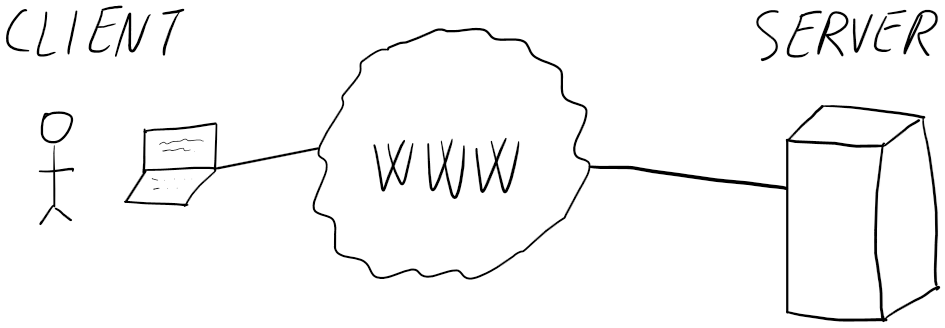
\includegraphics[width=0.5\linewidth]{Images/Client_server_connection_without_proxy.png}
	\caption{HTTP client server connection without proxy}
	\label{fig:connection_no_proxy}
\end{figure}

\begin{figure}
	\centering
	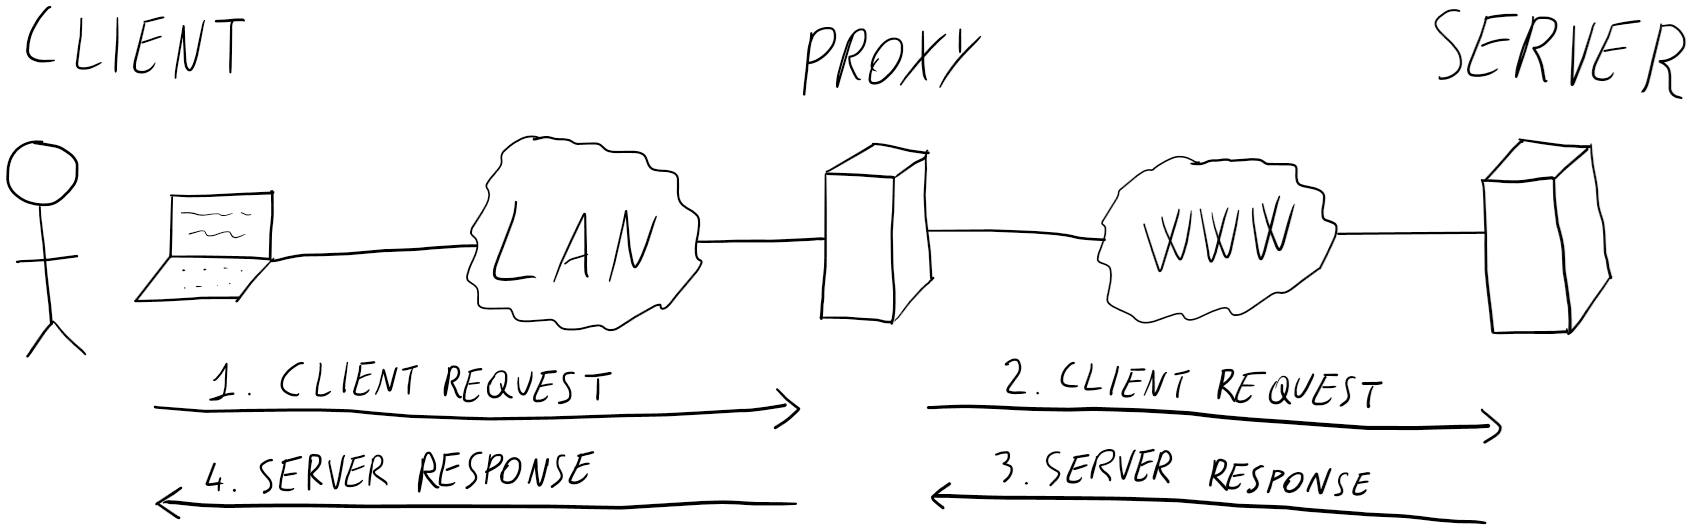
\includegraphics[width=\linewidth]{Images/Client_server_connection_with_proxy.png}
	\caption{HTTP client server connection with proxy}
	\label{fig:connection_with_proxy}
\end{figure}

A \textbf{proxy} (proximity machine) is an intermediary application that acts both as a server and as a client. Toward the original client, the proxy behaves as the endpoint that receives the request and may generate a response. Toward the origin server, or toward another intermediary, the same proxy behaves as a client and may forward the request.\\

In the classical case of a \textbf{forward proxy}, the proxy is part of the client-side access path (see figures \ref{fig:connection_no_proxy} and \ref{fig:connection_with_proxy}): the client is configured to send requests to the proxy, and therefore it is aware, at least at the HTTP or network configuration level, that it is not contacting the origin server directly. The proxy may then decide whether to satisfy the request locally or forward it. During this process it may perform transformation, control, verification, filtering, logging, access enforcement, or caching.\\

A proxy is not simply a mirror of the origin server. It can provide a resource to the client only when it is able to do so according to its role and its local state, for example because it owns a fresh cached copy. Otherwise, it must behave as a client toward the origin server or toward another intermediary in order to obtain the requested resource.\\

A different case is the \textbf{reverse proxy}. A reverse proxy is placed on the server side, in front of one or more origin servers. The client sends an ordinary request to what appears to be the server responsible for the resource, while the reverse proxy internally forwards the request to the appropriate backend server. From the client's perspective, a reverse proxy is therefore usually transparent and may look similar to a gateway. Its typical purposes include load balancing, caching, compression, TLS termination, request routing, protection of backend servers, and centralized logging.

\subsection{Gateway}

\begin{figure}
	\centering
	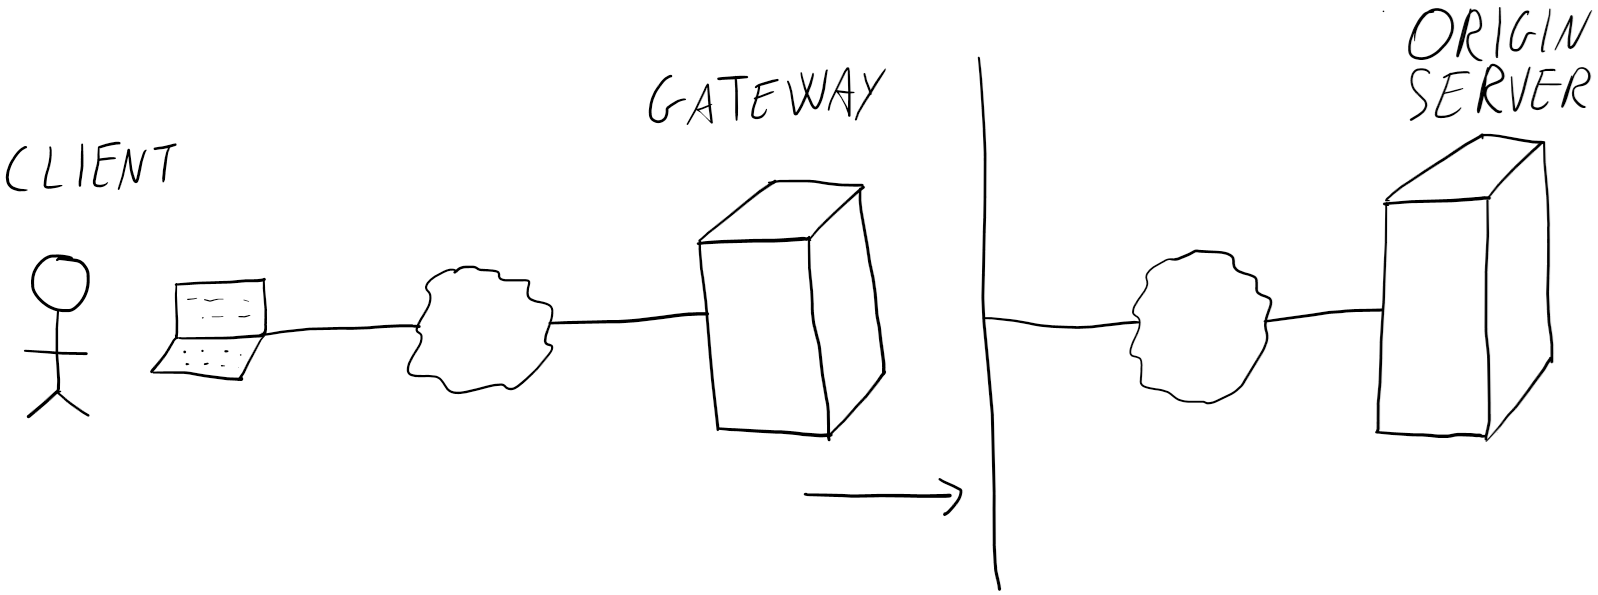
\includegraphics[width=\linewidth]{Images/Connection_with_gateway.png}
	\caption{HTTP client server connection with a gateway. The gateway receives the request on behalf of the origin server, analyzes it and decides whether to forward it to the origin server or not.}
	\label{fig:connection_with_gateway}
\end{figure}

A \textbf{gateway} is an intermediary application that acts on behalf of another server (see figure \ref{fig:connection_with_gateway}). Unlike a classical forward proxy, a gateway receives requests as if it were the origin server. The client may be unaware that the entity receiving the request is a gateway rather than the final server that owns, computes, or retrieves the resource.\\

This makes the gateway semantically close to the origin server from the client's perspective. The client addresses the gateway as the server responsible for the resource, while the gateway hides the internal organization behind that endpoint. A gateway can translate between protocols, connect different application environments, expose legacy systems through an HTTP interface, or provide a single HTTP-facing access point for resources managed elsewhere.\\

The distinction between proxy and gateway is therefore mainly one of \textbf{position and transparency}. A forward proxy is normally explicit from the client side, because the client deliberately uses it as an intermediary. A gateway is addressed as if it were the origin server. A reverse proxy is technically a proxy, but it shares the same client-side transparency as a gateway because it is deployed in front of the origin servers and hides the backend structure from the client.

\subsection{Tunnel}

A \textbf{tunnel} is an intermediary program that acts as a passive transmitter of HTTP-related traffic. It does not participate in the HTTP communication by interpreting or transforming the messages at the HTTP level, even though its creation may have been triggered by an HTTP connection.\\

Tunnels are useful when traffic must pass through an intermediate barrier without modifying that barrier's application-level behavior. Once established, the tunnel provides a forwarding path; it is not an HTTP participant in the same sense as a proxy or gateway.

\subsection{Cache}

A \textbf{cache} is both the local memory used to store previously obtained resources and the management system that controls their storage, validation, expiration, and update. Any client or server can use a cache.\\

Caching is a fundamental optimization in HTTP. It can reduce latency, network load, and server processing, provided that cached representations are kept coherent with the resources controlled by the origin server. In HTTP, caching is not merely a local implementation detail: the protocol includes headers and validation mechanisms that allow clients, servers, and intermediaries to reason about freshness, expiration, and revalidation.

\chapter{HTTP Message Structure and Core Methods}

\section{General Structure of HTTP Messages}

HTTP communication is based on messages exchanged according to the request-response model. A client sends a request message to ask the server to perform an action on a resource; the server returns a response message describing the outcome of that action and, when appropriate, carrying a representation of the requested resource.\\

The abstract syntax of an HTTP message can be expressed as follows. The symbols \texttt{CRLF} denote carriage return followed by line feed, \texttt{SP} denotes a blank space, and the vertical bar denotes an alternative.

\begin{lstlisting}
generic-message = start-line
                  *(message-header CRLF)
                  CRLF
                  [message-body]

start-line     = Request-Line | Status-Line

Request-Line   = Method SP Request-URI SP HTTP-Version CRLF

Status-Line    = HTTP-Version SP Status-Code SP Reason-Phrase CRLF

message-header = field-name ":" [field-value]

message-body   = entity-body
               | <entity-body encoded as per Transfer-Encoding>
\end{lstlisting}

The \texttt{start-line} determines the role of the message. In a request it is a \texttt{Request-Line}; in a response it is a \texttt{Status-Line}. The header section follows the start line and is composed of one header field per line. An empty line terminates the header section and separates it from the optional message body.\\

This organization is deliberately regular. The first line gives the immediate interpretation of the message, the header fields provide metadata and negotiation parameters, and the body carries the representation or data associated with the message when the method and the response semantics allow it.

\newpage
\section{HTTP Request Messages}

\begin{figure}[!h]
	\centering
	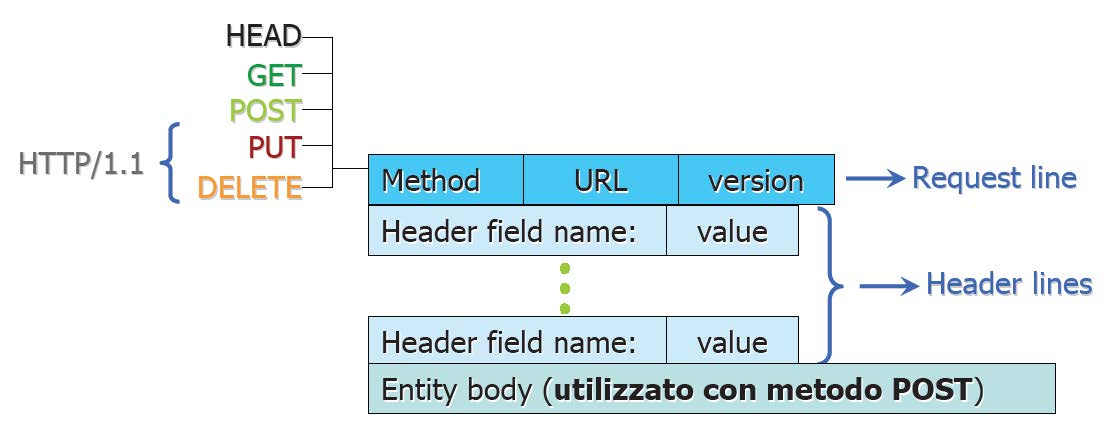
\includegraphics[width=\linewidth]{Images/HTTP_request_message.jpg}
	\caption{HTTP request message structure}
	\label{fig:HTTP_request_message}
\end{figure}

An HTTP request message starts with a request line. The request line contains the method, the resource identifier relative to the server context, and the HTTP version used by the client.

\begin{lstlisting}
Method SP Request-URI SP HTTP-Version CRLF
\end{lstlisting}

The \texttt{Method} specifies the action requested by the client. The \texttt{Request-URI} identifies the target resource, normally as a path interpreted with respect to the contacted server. The \texttt{HTTP-Version} expresses the version of the protocol that the client is using, such as \texttt{HTTP/1.0} or \texttt{HTTP/1.1}. If the request cannot be satisfied, the server still completes the request-response cycle by returning an appropriate response, rather than silently ignoring the message. In particular, the failure may depend on different causes: the method may be unsupported by the server, not allowed for the specific resource identified by the URI, or allowed only for clients satisfying suitable authentication and authorization requirements. These cases correspond to different response classes, such as \texttt{501 Not Implemented}, \texttt{405 Method Not Allowed}, \texttt{401 Unauthorized}, or \texttt{403 Forbidden}.\\

After the request line, the client may include header fields. Request headers can describe the client, the target host, the formats the client can process, authorization data, conditions for executing the method, and other metadata. The body, when present, is a MIME message carrying data sent from the client to the server. In typical HTTP usage, a \texttt{GET} request does not include a body, whereas methods such as \texttt{POST} and \texttt{PUT} are used when the client must transmit information content.

\newpage
\subsection{Example of a Request Message}

\begin{figure}[!h]
	\centering
	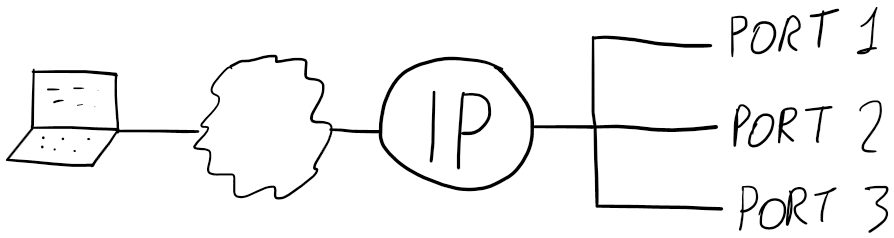
\includegraphics[width=\linewidth]{Images/Shared_hosting.png}
	\caption{Server shared hosting configuration. The different virtual sites are accessible using the same IP address but different ports.}
	\label{fig:shared_hosting}
\end{figure}

The following request asks for the resource \texttt{/index.html} using HTTP/1.1 and includes several request-specific headers.

\begin{lstlisting}
	GET /index.html HTTP/1.1
	Referer: http://www.poliba.it/pippo.html
	User-Agent: Mozilla/4.61
	Host: www.microsoft.com:80
	Accept: image/gif, image/jpeg, image/png, */*
	Accept-Encoding: gzip
	Accept-Language: it
	Accept-Charset: iso-8859-1,*,utf-8
\end{lstlisting}

The request line states that the client wants to retrieve \texttt{/index.html}. The \texttt{Host} header specifies the domain name and port associated with the request, which is essential in HTTP/1.1 when several virtual sites may share the same network endpoint (see figure \ref{fig:shared_hosting}). The \texttt{User-Agent} header identifies the client software, while \texttt{Referer} indicates the page from which the user reached the requested resource.\\

The \texttt{Accept} family of headers expresses the representations that the client is able or willing to process. In the example, the client declares that it can accept \texttt{image/gif}, \texttt{image/jpeg}, and \texttt{image/png}. The wildcard \texttt{*/*} means that other media types are not excluded a priori. The \texttt{Accept-Encoding} header indicates that the client can process a response compressed with \texttt{gzip}. The \texttt{Accept-Language} header expresses a preference for Italian content, while \texttt{Accept-Charset} lists acceptable character sets and includes a wildcard alternative. These fields allow the server to select a representation that is compatible with the capabilities and preferences of the client.\\

Client preferences may be refined through \textbf{quality factors}. A quality factor is expressed by the parameter \texttt{q} and has a value between \texttt{0} and \texttt{1}. A value of \texttt{1} denotes the highest preference, while \texttt{0} means that the corresponding representation is not acceptable. For example:

\begin{lstlisting}
Accept: image/png;q=1.0, image/jpeg;q=0.8, image/gif;q=0.6, */*;q=0.1
Accept-Language: it;q=1.0, en;q=0.7
Accept-Charset: iso-8859-1;q=1.0, utf-8;q=0.8, *;q=0.5
\end{lstlisting}

In this case, if several representations of the same resource are available, the server should prefer \texttt{image/png} over \texttt{image/jpeg}, \texttt{image/jpeg} over \texttt{image/gif}, and any explicitly listed image format over the generic wildcard. The wildcard is not automatically a last-resort option because it appears at the end of the list; it becomes a low-priority option because its quality factor is lower. Conversely, a wildcard with a high quality factor could be preferred over a more specific format with a lower quality factor, depending on the applicable negotiation rules and on the representations actually available on the server.\\

When quality factors are omitted, their default value is \texttt{1}. Therefore, in the original request:

\begin{lstlisting}
Accept: image/gif, image/jpeg, image/png, */*
Accept-Charset: iso-8859-1,*,utf-8
\end{lstlisting}

all listed alternatives have the same explicit preference from the client's point of view. The server is then free to choose among the compatible representations according to its own selection policy, the available resource variants, and the specificity of the match. In general, a specific media range such as \texttt{image/png} is more informative than a wildcard such as \texttt{*/*}, but without quality factors the client is not expressing a strict priority order among the listed alternatives. Quality factors are therefore the mechanism used to make the preference order explicit and to reduce ambiguity during server-driven content negotiation.

\section{Request Methods}

HTTP methods define the operation that the client wants the server to apply to the target resource. The most important methods are \texttt{GET}, \texttt{HEAD}, \texttt{POST}, and \texttt{PUT}. Other methods, used more rarely in ordinary Web interactions, include \texttt{OPTIONS}, \texttt{DELETE}, \texttt{TRACE}, and \texttt{CONNECT}.\\

Two properties are useful for classifying methods:
\begin{itemize}
    \item a method is \textbf{safe} when executing it does not request a change in the internal state of the server;
    \item a method is \textbf{idempotent} when the intended effect of repeated identical requests is the same as the effect of a single request.
\end{itemize}

These properties are semantic guarantees about the requested operation, not about the absence of secondary effects such as logging, monitoring, or accounting. They are important because clients, proxies, caches, and retry mechanisms may use them to decide whether a request can be repeated, optimized, or validated without changing the resource state.

\subsection{GET}

\texttt{GET} is the most frequently used HTTP method and was the only method available in HTTP/0.9. It requests a representation of a resource from the server. In its ordinary form, the server returns the selected representation in the response body.\\

\texttt{GET} is safe and idempotent. It can appear in three relevant forms:
\begin{itemize}
    \item \textbf{absolute}, when the resource is requested without additional conditions;
    \item \textbf{conditional}, when the request must be executed only if conditions expressed in header fields hold, for example through \texttt{If-Match}, \texttt{If-Modified-Since}, or \texttt{If-Range};
    \item \textbf{partial}, when the client requests only a subpart of a stored resource, typically by using byte ranges.
\end{itemize}

Conditional and partial requests are central to efficient resource transfer. A conditional request avoids sending a representation when the client already owns an up-to-date copy. A partial request is useful when only a segment of a resource is needed (see figure \ref{fig:web_page_structure}) or when a transfer has to resume after interruption.

\begin{figure}
	\centering
	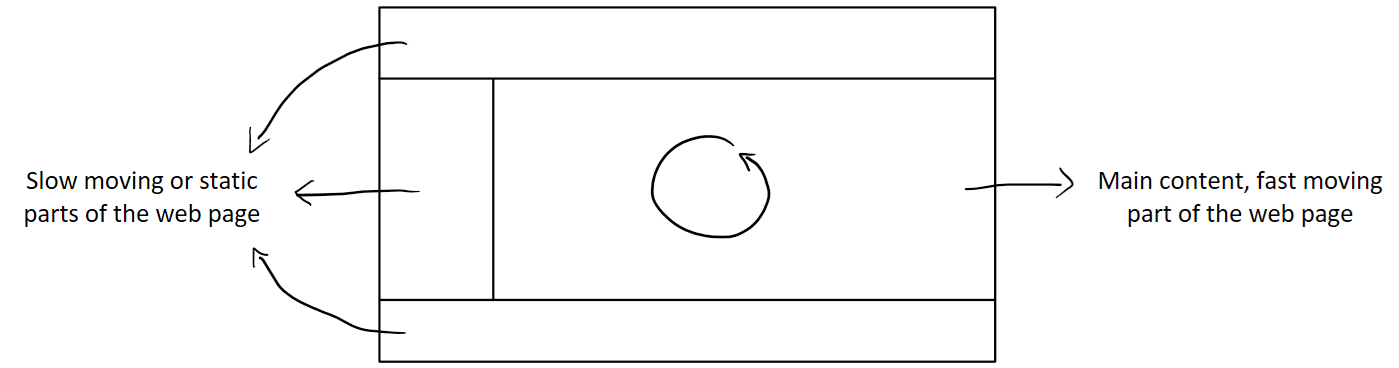
\includegraphics[width=\linewidth]{Images/Web_page_structure.png}
	\caption{Structure of a web page with labels distinguishing the static or slow moving part of the page from the fast moving content of the page. In this case, it is possible to use partial GET requests to download only the page content instead of the whole page.}
	\label{fig:web_page_structure}
\end{figure}

\subsubsection{GET and Form Submission}

Web forms can use \texttt{GET} as their submission method. In that case, the form fields are encoded in the query string of the requested URI. As an example, let us consider the following form:

\begin{lstlisting}
<form method="GET" action="foo.php">
  First Name: <input type="text" name="first_name" /> <br/>
  Last Name: <input type="text" name="last_name" /> <br/>
	
  <input type="submit" name="action" value="Submit" />
</form>
\end{lstlisting}

Submitting a form with the fields \texttt{first\_name}, \texttt{last\_name}, and \texttt{action} may produce a request line such as:

\begin{lstlisting}
GET /foo.php?first_name=Mario&last_name=Rossi&action=Submit HTTP/1.1
\end{lstlisting}

This form of submission makes the transmitted parameters part of the URI. It is appropriate for retrieval-oriented operations, where the submitted data identifies or filters the requested representation rather than creating or modifying server-side state. It is \textbf{inappropriate for sensitive information} such as passwords because it would be transferred in plain text through the URL.

\newpage
\subsection{HEAD}

\texttt{HEAD} is similar to \texttt{GET}, but the server returns only the header section and omits the response body. The metadata returned by \texttt{HEAD} should describe the same resource that would have been returned by a corresponding \texttt{GET} request.\\

\texttt{HEAD} is safe and idempotent. It is commonly used to verify:
\begin{itemize}
    \item the \textbf{validity} of a URI, namely whether the resource exists and is not a zero-length placeholder;
    \item the \textbf{accessibility} of a URI, namely whether the resource can be obtained directly or whether an authentication procedure is required;
    \item the \textbf{cache coherence} of a URI, by checking metadata such as modification date, length, hash, or validation information.
\end{itemize}

The method is useful when the client or an intermediate cache needs information about a resource without transferring the resource representation itself. For example, a cache can issue a \texttt{HEAD} request to compare the last modification date or content length of a stored representation with the current metadata known by the origin server. If the cached representation is still coherent, a subsequent \texttt{GET} is unnecessary. If the metadata shows that the representation has changed, the cache can perform a normal retrieval.\\

This strategy trades an additional lightweight request-response exchange for a possible reduction in bandwidth and server-side processing. It is particularly useful when resources are large and modifications are relatively infrequent.

\subsection{PUT}

\texttt{PUT} transmits information from the client to the server in order to create or replace the resource identified by the request URI. The representation sent with \texttt{PUT} is, in general, the representation that the client expects to obtain later by making a \texttt{GET} request on the same URI.\\

\texttt{PUT} is idempotent but not safe. Repeating the same \texttt{PUT} request has the same intended effect as executing it once, because the target resource is created or replaced with the same representation. However, the method changes the internal state of the server, and therefore it cannot be considered safe.\\

The method semantics do not by themselves provide access control or locking. A server that accepts \texttt{PUT} must therefore rely on additional mechanisms to decide who is authorized to create or replace a resource and how concurrent updates are coordinated.

\subsection{DELETE}

\texttt{DELETE} requests the removal of the resource identified by the target URI from the Web server. It changes server-side state and is therefore not safe.\\

Deletion is operationally delicate because it affects the availability of the resource for subsequent requests. After a successful deletion, later requests for the same URI may fail because the selected resource is no longer present. This is relevant in concurrent settings, where more than one client or process may attempt to delete or access the same resource in overlapping time intervals. For this reason, implementations must combine \texttt{DELETE} with suitable authorization and consistency policies.

\subsection{POST}

\texttt{POST} sends subordinate or additional information from the client to the server, usually in relation to an existing resource. Typical examples include adding a database record, posting a message to a forum or newsgroup, uploading a file into a directory, or submitting form data edited by a user.\\

\texttt{POST} is neither safe nor idempotent. It changes server-side state, and repeated identical \texttt{POST} requests may create multiple subordinate resources or append the same information multiple times.\\

A server can respond positively to a \texttt{POST} request in several ways:
\begin{itemize}
    \item \texttt{200 OK}, when the data has been received and processed, and the response contains a body;
    \item \texttt{201 Created}, when the data has been received and a new resource has been created;
    \item \texttt{204 No Content}, when the data has been received and processed, but the response does not contain a body.
\end{itemize}

The distinction between \texttt{PUT} and \texttt{POST} is therefore not simply that both transmit data to the server. With \texttt{PUT}, the client addresses the resource to create or replace. With \texttt{POST}, the client submits information to be processed in the context of another resource, and the server determines the precise effect.

\section{HTTP Response Messages}

\begin{figure}[!h]
	\centering
	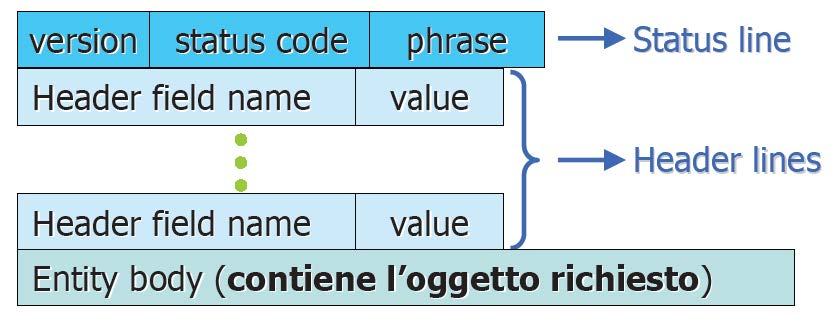
\includegraphics[width=0.5\linewidth]{Images/HTTP_response_message.jpg}
	\caption{HTTP response message}
	\label{fig:HTTP_response_message}
\end{figure}

An HTTP response message begins with a status line. The status line contains the HTTP version, a numeric status code, and a reason phrase.

\begin{lstlisting}
HTTP-Version SP Status-Code SP Reason-Phrase CRLF
\end{lstlisting}

The header section follows the status line and describes the response, the server, and the representation contained in the body. The response body, when present, carries the entity returned to the client. For a successful retrieval, this body contains the requested representation; for some responses, such as \texttt{204 No Content}, it is deliberately absent.

\subsection{Example of a Response Message}

The following response reports a successful request and returns an HTML entity.

\begin{lstlisting}
HTTP/1.1 200 OK
Date: Fri, 11 Mar 2005 11:42:03 GMT
Server: Apache/1.3.3
Last-Modified: Tue, 1 Feb 2005 08:21:02 GMT
Content-Length: 127
Content-Type: text/html

<HTML> ... </HTML>
\end{lstlisting}

The status line states that the server is using \texttt{HTTP/1.1} and that the request succeeded with status code \texttt{200}. The \texttt{Date} header indicates the transmission time. The \texttt{Server} header identifies the server software. The \texttt{Last-Modified} field gives metadata useful for validation and cache coherence. The \texttt{Content-Length} and \texttt{Content-Type} headers describe the body: its length in bytes and its MIME type.

\section{Status Codes}

The status code is a three-digit number. The first digit identifies the class of the response, while the remaining digits specify the concrete condition within that class.

\begin{center}
\begin{tabular}{p{0.18\textwidth}p{0.72\textwidth}}
\textbf{Class} & \textbf{Meaning} \\
\hline
\texttt{1xx} & Informational response. It indicates a provisional response, for example while the request is still being completed. \\ \hline

\texttt{2xx} & Successful response. The client's request was successfully received, understood, and served. \\ \hline

\texttt{3xx} & Redirection response. The request was received and understood, but the user agent must perform further action to complete it. \\ \hline

\texttt{4xx} & Client error. The request cannot be satisfied because of a client-side problem, such as a syntax error or lack of authorization. \\ \hline

\texttt{5xx} & Server error. The request may be correct, but the server is unable to satisfy it because of an internal error or an application-side failure. \\ \hline
\end{tabular}
\end{center}

Status codes allow the server to preserve the request-response structure even when the requested action cannot be completed. For example, a syntactically invalid request does not simply disappear; it is answered with a status code in the \texttt{4xx} family. A method that the server does not support is answered with a server-side capability error.

\newpage
\subsection{Representative Status Codes}

The following codes illustrate the main classes and the corresponding reason phrases:

\begin{table}[!h]
	\begin{tabularx}{\linewidth}{p{0.4\textwidth}X}
	\textbf{Code} & \textbf{Typical meaning} \\
	\hline
	
	\texttt{100 Continue} & The client may continue, for example when it has not yet sent the request body. \\ \hline
	
	\texttt{200 OK} & Successful request, typically a successful \texttt{GET}. \\ \hline
	
	\texttt{201 Created} & Successful creation of a resource, for example after a successful \texttt{PUT}. \\ \hline
	
	\texttt{301 Moved Permanently} & The requested URL is no longer the current location, and the server knows the new resource location. \\ \hline
	
	\texttt{400 Bad Request} & The request contains a syntax error. \\ \hline
	
	\texttt{401 Unauthorized} & The request lacks the authorization required to access the resource. \\ \hline
	
	\texttt{403 Forbidden} & The server refuses to fulfill the request. \\ \hline
	
	\texttt{404 Not Found} & The requested URL does not identify an available resource. \\ \hline
	
	\texttt{500 Internal Server Error} & The server encountered an internal failure, often related to server-side application logic. \\ \hline
	
	\texttt{501 Not Implemented} & The server does not support the requested method. \\ \hline
	\end{tabularx}
\end{table}

The reason phrase is a textual explanation associated with the numeric code. Protocol logic should rely on the numeric code, because the class and the precise condition are encoded there. The phrase is primarily intended to make the response easier to interpret for humans and diagnostic tools.

\chapter{HTTP Header Fields and Content Negotiation}

\section{Role of the Header Section}

The header section is the part of an HTTP message that follows the request line in a request message or the status line in a response message. It is terminated by an empty line, which separates metadata from the optional message body.\\

The start line gives only the immediate interpretation of the message: the method and target resource in a request, or the status code in a response. The header section carries the detailed information needed to process the message correctly. It describes the transmission, the representation carried in the body, the request made by the client, or the response produced by the server.\\

A header section is a sequence of header fields. Each field is a key--value element whose name is defined by the protocol and whose value provides the concrete metadata for the current message.

\begin{lstlisting}
field-name: field-value
\end{lstlisting}

Header names are written as single lexical units. When a name contains several words, HTTP conventionally uses hyphens, as in \texttt{Content-Type}, \texttt{User-Agent}, or \texttt{If-Modified-Since}. A blank space would be interpreted as a separator and would not be part of the header field name.\\

HTTP header fields can be grouped according to the kind of information they express:
\begin{itemize}
    \item \textbf{generic headers}, which refer to the transmitted message and may appear in both requests and responses;
    \item \textbf{entity-based headers}, which describe the message body or, if no body is present, the resource associated with the message;
    \item \textbf{request-specific headers}, which are set by the client to describe the request and the client-side capabilities;
    \item \textbf{response-specific headers}, which are set by the server to describe the response and the server-side capabilities.
\end{itemize}

This classification is useful because HTTP messages are structurally simple but semantically rich. Most of the protocol behavior is not expressed in the start line, but in the metadata attached to it.

\section{MIME and Representation Metadata}

HTTP uses MIME-style metadata to describe the format and processing requirements of transferred contents. MIME, \emph{Multipurpose Internet Mail Extensions}, was originally introduced for electronic mail, where the early infrastructure was essentially oriented toward textual content. In fact, the SMTP-based systems used to deliver correctly only the first 128 combinations of the ASCII code because those combinations represent the alphanumeric characters. Binary files, images, and other non-textual objects required an explicit classification and encoding mechanism because their bytes may use the whole range of possible byte values, not only the values safely handled by text-oriented mail systems.\\

The same idea is used in HTTP to classify Web representations. Each data stream is associated with a content type written as an object/format pair:

\begin{lstlisting}
Content-Type: object/format
\end{lstlisting}

The first component identifies the general kind of content, such as \texttt{text}, \texttt{image}, \texttt{audio}, or \texttt{application}. The second component identifies the concrete format used for that object. For example, a textual object may be represented as \texttt{text/plain} or \texttt{text/html}; an image may be represented as \texttt{image/jpeg} or \texttt{image/png}.\\

Every object/format pair is a MIME type, also called a content type. The official list of standard MIME types is managed by the Internet Assigned Numbers Authority. When a representation does not match a standardized type, the generic type \texttt{application/octet-stream} can be used to indicate an arbitrary sequence of bytes. This does not give the recipient detailed semantic information, but it allows the transfer to be classified as binary application data.

\subsection{Content Type and Transfer Encoding}

The content type describes what the entity is. Encoding metadata describes how it has been encoded for transmission or processing. This distinction is relevant because the same conceptual object may be transferred in different encoded forms.\\

For example, the following field classifies the body as a JPEG image:

\begin{lstlisting}
Content-Type: image/jpeg
\end{lstlisting}

By contrast, the following field indicates that the transferred object is encoded in Base64 form:

\begin{lstlisting}
Content-Transfer-Encoding: base64
\end{lstlisting}

The two fields answer different questions. \texttt{Content-Type} specifies the type and format of the represented object. \texttt{Content-Transfer-Encoding} specifies the encoding used to transmit that object. MIME defines several standard encodings, including \texttt{7bit}, \texttt{quoted-printable}, and \texttt{base64}. Correct processing requires both kinds of information when the representation is not directly usable in its transmitted form.

\newpage
\section{Generic Header Fields}

Generic headers apply to the transmitted message itself. They are not specific to requests or responses and may appear in either direction.

\begin{table}[!h]
	\begin{tabularx}{\linewidth}{p{0.25\textwidth}X}
	\textbf{Header field} & \textbf{Purpose} \\
	\hline
	\texttt{Date} & Date and time at which the message is transmitted. It is useful for freshness, diagnostics, and temporal checks. \\ \hline
	
	\texttt{MIME-Version} & MIME version used for the transmission. In this context the value is normally \texttt{1.0}. \\ \hline
	
	\texttt{Transfer-Encoding} & Encoding applied to the message for transfer. The receiver must interpret this information to recover the transferred representation correctly. \\ \hline
	
	\texttt{Cache-Control} & Directives that specify or suggest the caching mechanism to apply to the resource or message. \\ \hline
	
	\texttt{Connection} & Desired behavior of the connection, such as keeping it active or closing it after the response. \\ \hline
	
	\texttt{Via} & Information inserted by proxies or gateways to indicate that the message has passed through an intermediary. \\ \hline
	\end{tabularx}
\end{table}

The \texttt{Connection} header is particularly relevant because it links message metadata with connection management. In older HTTP interactions, the default behavior was to close the connection after the request-response exchange. With persistent connections, a client or server can use connection metadata to indicate whether the connection should remain available for subsequent exchanges.\\

The \texttt{Via} header is relevant in architectures where the client is not communicating directly with the origin server. A proxy or gateway can insert this field to make the presence of an intermediary explicit in the message path.

\newpage
\section{Entity-Based Header Fields}

Entity-based headers describe the message body. If the message has no body, they may describe the selected resource rather than an actual transferred payload. Their purpose is to make the representation processable by the recipient and manageable by caches.

\begin{table}[!h]
	\begin{tabularx}{\linewidth}{p{0.25\textwidth}X}
	\textbf{Header field} & \textbf{Purpose} \\
	\hline
	
	\texttt{Content-Type} & MIME type of the entity. It is mandatory when a message contains a body. \\ \hline
	
	\texttt{Content-Length} & Length of the body in bytes. It is mandatory when a message contains a body and the body length must be explicitly known. \\ \hline
	
	\texttt{Content-Encoding} & Encoding applied to the entity representation. \\ \hline
	
	\texttt{Content-Language} & Natural language associated with the entity. \\ \hline
	
	\texttt{Content-Location} & URL associated with the supplied representation. \\ \hline
	
	\texttt{Content-MD5} & MD5 value associated with the entity, used as an integrity-related metadata field. \\ \hline
	
	\texttt{Content-Range} & Range of the resource represented in the current message. \\ \hline
	
	\texttt{Expires} & Date after which the resource is considered no longer valid and must be revalidated or removed from cache. \\ \hline
	
	\texttt{Last-Modified} & Date and time of the last modification of the resource; useful for deciding whether a cached copy is still valid. \\ \hline
	\end{tabularx}
\end{table}

These fields avoid unnecessary or unusable transfers. A client may receive the correct resource identifier but in a format it cannot process; conversely, a server may accept a request body only if it can interpret its representation. Entity metadata therefore supports both interoperability and efficiency.\\

The \texttt{Expires} and \texttt{Last-Modified} fields are also central to cache management. \texttt{Expires} gives an explicit freshness limit. \texttt{Last-Modified} supports validation, because a client or proxy can compare the version it owns with the version available at the origin server.

\section{Request-Specific Header Fields}

Request-specific headers are set by the client. They describe the client software, the target host, the context of navigation, the requested representation, and conditions under which the server should execute the method.

\subsection{Client and Navigation Metadata}

The \texttt{User-Agent} header contains a string describing the client that originates the request. A typical value includes the client family, version, compatibility information, and the operating system. Although modern Web applications are expected to be broadly compatible with standard browsers, the field remains useful for diagnostics, adaptation, and handling complex applications that depend on specific client capabilities.

\begin{lstlisting}
User-Agent: Mozilla/4.61 (compatible; MSIE 6.0; Windows NT 5.1; SV1)
\end{lstlisting}

The \texttt{Referer} header contains the URL of the page from which the user reached the requested URL. The historical spelling \texttt{Referer} is part of the protocol terminology, even though the ordinary English word would be \emph{referrer}. If the user requests a URL directly, for example by typing it or selecting it from bookmarks, this header must be absent.

\begin{lstlisting}
Referer: http://www.poliba.it/pippo.html
\end{lstlisting}

This field can be useful for understanding navigation flows, but it also has privacy implications. Since it reveals the previous page, it can be used for profiling, analytics, or advertising-oriented tracking. Its use must therefore be considered carefully in systems that process user-related information.

\subsection{Host Identification and Virtual Hosting}

The \texttt{Host} header specifies the domain name and port to which the connection is made. It is mandatory in HTTP/1.1.

\begin{lstlisting}
Host: www.example.org:80
\end{lstlisting}

This field enables name-based virtual hosting, also called multi-homing in this context. Several Web sites can be served by the same physical machine and the same IP address. The network connection reaches the machine, but the \texttt{Host} header tells the HTTP server which logical site the request addresses. This avoids requiring a distinct IP address for every hosted Web site and does not require routing-level manipulation.

\subsection{User Identity and Authorization Metadata}

The \texttt{From} header may contain the email address of the requester. In practice, it is rarely used because it exposes personal information. It should be inserted only with the user's approval.

\begin{lstlisting}
From: user@example.org
\end{lstlisting}

The \texttt{Authorization} and \texttt{Proxy-Authorization} headers carry authorization information for accessing a restricted resource or for authenticating to a proxy. The exact content of these fields depends on the authentication mechanism in use.

\begin{lstlisting}
Authorization: <authorization-data>
Proxy-Authorization: <authorization-data>
\end{lstlisting}

These headers are part of the request because the server or proxy must evaluate access rights before returning the protected representation.

\subsection{Partial Resource Requests}

The \texttt{Range} header allows the client to request only a specified byte interval of a resource instead of the entire representation.

\begin{lstlisting}
Range: bytes=500-999
\end{lstlisting}

This mechanism is especially useful when resuming interrupted downloads or when only a portion of a large resource is needed. It reduces traffic by avoiding the retransmission of bytes that the client already owns. It also supports the practical case in which different parts of a large resource change at different rates and the client needs only a selected portion.\\

The server communicates its support for range requests through response metadata, especially \texttt{Accept-Ranges}. If the server cannot provide ranges, it may require the client to retrieve the whole resource.

\section{Content Negotiation}

HTTP content negotiation allows the client to state which representations it can process. The server then selects the best available representation of the target resource. This is necessary because the same resource may be available in several MIME types, character sets, transfer encodings, or natural languages.\\

The main request headers involved are:
\begin{itemize}
    \item \texttt{Accept}, for MIME types;
    \item \texttt{Accept-Charset}, for character sets;
    \item \texttt{Accept-Encoding}, for encodings;
    \item \texttt{Accept-Language}, for natural languages.
\end{itemize}

A client can specify several acceptable alternatives in a comma-separated list.

\begin{lstlisting}
Accept: text/html, application/xml
\end{lstlisting}

When no explicit preference is specified, the server may choose among the acceptable alternatives according to its own configuration or defaults. When the client wants to rank alternatives, it uses the \texttt{q} parameter, also called the relative quality factor.

\subsection{Quality Factors}

A quality factor is a value between \texttt{0} and \texttt{1}. The value \texttt{1} represents the highest preference and is the default when no \texttt{q} value is specified; \texttt{0} represents the lowest preference.

\begin{lstlisting}
Accept: text/html, text/x-c, text/x-dvi;q=0.8, text/plain;q=0.5
\end{lstlisting}

This header states that the client prefers \texttt{text/html} and \texttt{text/x-c}. If neither is available, it can accept \texttt{text/x-dvi}; if that is not available, it can still accept \texttt{text/plain}. The order of the comma-separated entries is not the reliable way to express a preference. The preference is expressed by the quality factor.\\

Wildcards can be used when the client is willing to accept a broader family of representations. The form \texttt{image/*} accepts every image format supported by the server. The form \texttt{*/*} accepts every object in every format.

\begin{lstlisting}
Accept: text/html, application/xml;q=0.9, */*;q=0.8
\end{lstlisting}

This means that the client prefers \texttt{text/html}; if it is unavailable, it prefers \texttt{application/xml}; if neither is available, it can accept another representation. The wildcard is not merely a syntactic backup placed at the end of the list. It participates in the same selection mechanism and must be interpreted together with the quality factors.\\

The same mechanism applies to character sets and encodings.

\begin{lstlisting}
Accept-Charset: iso-8859-1, *;q=0.8, utf-8
Accept-Encoding: gzip
Accept-Language: it
\end{lstlisting}

The purpose of this negotiation is not only user preference. It also prevents useless traffic. If the server sends a representation that the client cannot decode or process, bandwidth and server processing have been wasted. By declaring acceptable formats in advance, the client allows the server to select a representation that is both available and usable.

\section{Conditional Requests}

Conditional request headers allow the client to ask the server to execute a method only if a stated condition is true. They are especially useful for cache validation.\\

The headers \texttt{If-Modified-Since} and \texttt{If-Unmodified-Since} use HTTP timestamp values. The timestamp syntax follows the date formats used by Internet message specifications.

\begin{lstlisting}
If-Modified-Since: Wed, 21 Oct 2015 07:28:00 GMT
If-Unmodified-Since: Wed, 21 Oct 2015 07:28:00 GMT
\end{lstlisting}

The general idea is that the request is evaluated against the current state of the target resource. If the condition is relevant and the resource state satisfies it, the method is performed. If the condition is not satisfied, the server avoids sending an unnecessary representation or rejects the operation according to the semantics of the condition.\\

For cache validation, the typical case is \texttt{If-Modified-Since}. A client or proxy that owns a cached copy asks the server whether the resource has changed after the specified date. If the resource has been modified, the server returns \texttt{200 OK} and sends the updated representation in the body. If the resource has not been modified, the server returns \texttt{304 Not Modified} and does not send the body.

\begin{lstlisting}
GET /index.html HTTP/1.1
Host: www.example.org
If-Modified-Since: Wed, 21 Oct 2015 07:28:00 GMT
\end{lstlisting}

If the request would produce a response different from \texttt{200 OK} even without the condition, or if the date is not valid, the conditional header is ignored. This prevents conditional metadata from hiding more fundamental errors, such as an invalid request or an inaccessible resource.\\

Conditional requests reduce the number of full transfers. Compared with an explicit preliminary \texttt{HEAD} request followed by a possible \texttt{GET}, a conditional \texttt{GET} can validate the cached copy and retrieve the new representation only when needed.

\newpage
\section{Response-Specific Header Fields}

Response-specific headers are inserted by the server. They describe the response, the server application, and the constraints or capabilities associated with the returned resource.

\begin{table}[!h]
	\begin{tabularx}{\linewidth}{p{0.25\textwidth}X}
	\textbf{Header field} & \textbf{Purpose} \\
	\hline
	
	\texttt{Server} & String describing the server, typically including the server type, version, and sometimes the operating system. \\ \hline
	
	\texttt{Accept-Ranges} & Kind of byte range the server accepts for the resource. Expected values include \texttt{bytes} and \texttt{none}. \\ \hline
	
	\texttt{WWW-Authenticate} & Authentication criteria required to access a restricted resource. It is used together with an authorization challenge. \\ \hline
	\end{tabularx}
\end{table}

The \texttt{Server} field is mainly diagnostic, but it may also reveal implementation details. The \texttt{Accept-Ranges} field is relevant when the client wants to resume downloads or request only a part of a resource. The \texttt{WWW-Authenticate} field is returned when the server requires authentication before granting access to the requested resource, typically together with a \texttt{401 Unauthorized} response.\\

Together, request-specific and response-specific headers make HTTP negotiation explicit. The client describes what it can accept and under which conditions it wants the method to be executed; the server describes what it produced, how it should be interpreted, and which additional requirements apply.

\chapter{HTTP Authentication, Connections, and Session Management}

\section{Restricted Resources and HTTP Authentication}

HTTP authentication is based on a challenge-response interaction. When a client requests a resource whose access is restricted, the server does not immediately return the representation. Instead, it answers with a response indicating that authorization is required and specifies the authentication scheme and the parameters that the client must use.\\

The typical first response is \texttt{401 Unauthorized}. The response includes the \texttt{WWW-Authenticate} header field, which describes the authentication challenge. A subsequent request from the client includes an \texttt{Authorization} header field containing the credentials or the computed authentication data required by the selected scheme.

\begin{lstlisting}
GET /private/index.html HTTP/1.1
Host: www.example.org

HTTP/1.1 401 Unauthorized
WWW-Authenticate: Basic realm="Restricted area"
\end{lstlisting}

The authentication information is therefore not part of the request line. It is carried by headers, consistently with the general role of the header section: the start line states the requested action and target resource, while headers describe the conditions under which the action can be performed.\\

HTTP defines two classical authentication mechanisms:
\begin{itemize}
    \item \textbf{Basic access authentication}, introduced with HTTP/1.0;
    \item \textbf{Digest access authentication}, introduced with HTTP/1.1.
\end{itemize}

Both mechanisms are tied to the notion of a \textbf{realm}. A realm is a security context grouping resources protected by the same access policy. Once the user agent has obtained credentials for a realm, it can reuse the corresponding authentication header for subsequent requests to resources belonging to the same realm.

\subsection{Credential Collection After an HTTP Authentication Challenge}

When a server replies with \texttt{401 Unauthorized} and includes a \texttt{WWW-Authenticate} header, the user agent is responsible for obtaining the credentials required by the selected authentication scheme. In the case of a browser, this normally produces a native authentication dialog asking for a username and a password. The dialog is not part of the HTML document and is not created by JavaScript; it is generated by the browser as a consequence of the HTTP authentication challenge.\\

For example, after the browser receives the following response:

\begin{lstlisting}
HTTP/1.1 401 Unauthorized
WWW-Authenticate: Basic realm="Restricted Area"
\end{lstlisting}

it may display a built-in dialog associated with the site and with the realm
\texttt{Restricted Area}. Once the user inserts the credentials, the browser
repeats the request and adds an \texttt{Authorization} header:

\begin{lstlisting}
GET /private/index.html HTTP/1.1
ost: www.example.org
Authorization: Basic YWxpY2U6c2VjcmV0
\end{lstlisting}

The average user does not need to know the structure of the HTTP exchange. The browser translates the protocol-level challenge into an authentication dialog and then constructs the second request. If the credentials are valid, the server returns the requested representation. If they are invalid, the server may return another \texttt{401 Unauthorized} response and repeat the challenge.\\

This behavior is specific to HTTP authentication. If a server returns a bare \texttt{401 Unauthorized} response without a usable challenge, or if the browser does not present an authentication dialog, the user cannot infer a standard place where credentials must be inserted. In such a case, the resource may be intended for programmatic clients, may require a different authentication mechanism, or may simply not expose a user-facing login interface.

\subsection{Application-Level Redirection to Login Pages}

Most modern web applications do not use the browser-native dialog associated with HTTP Basic or Digest authentication for ordinary user login. Instead, they implement authentication at the application level. In that case, the protected resource is still requested through HTTP, but the credential collection is managed by the application through an HTML form, a JavaScript interface, or an API endpoint.\\

A common interaction is based on redirection. When an unauthenticated user requests a protected page, the application does not necessarily answer with an HTTP authentication challenge. It may instead redirect the browser to a login page:

\begin{lstlisting}
GET /reserved/dashboard HTTP/1.1
Host: www.example.org

HTTP/1.1 302 Found
Location: /login?next=/reserved/dashboard
\end{lstlisting}

The browser follows the redirection and requests the login page:

\begin{lstlisting}
GET /login?next=/reserved/dashboard HTTP/1.1
Host: www.example.org

HTTP/1.1 200 OK
Content-Type: text/html
\end{lstlisting}

The user then sees a normal web page containing a login form. After the form is submitted, the application verifies the credentials, usually against an application database or an external identity provider. If the authentication succeeds, the application creates a session, commonly represented by a cookie, and redirects the browser back to the originally requested resource:

\begin{lstlisting}
POST /login HTTP/1.1
Host: www.example.org
Content-Type: application/x-www-form-urlencoded

username=alice&password=secret

HTTP/1.1 303 See Other
Set-Cookie: session=abc123; HttpOnly; Secure
Location: /reserved/dashboard
\end{lstlisting}

The status code \texttt{303 See Other} is well suited after a successful form submission because it instructs the user agent to perform a subsequent \texttt{GET} request to the URI given in the \texttt{Location} header. This avoids repeating the original \texttt{POST} request if the user refreshes the resulting page. In practice, \texttt{302 Found} is also widely used for this kind of login redirection, especially in older applications and frameworks.\\

The subsequent request contains the session cookie:

\begin{lstlisting}
GET /reserved/dashboard HTTP/1.1
Host: www.example.org
Cookie: session=abc123
\end{lstlisting}

At this point, the application recognizes the session and can decide whether the user is allowed to access the requested resource.\\

The main redirection cases related to authentication are therefore the following:

\begin{itemize}
	\item an unauthenticated browser request for a protected application page
	may receive \texttt{302 Found} or \texttt{303 See Other} with a
	\texttt{Location} header pointing to a login page;
	
	\item after a successful login submitted through \texttt{POST}, the server
	commonly returns \texttt{303 See Other}, or sometimes \texttt{302 Found},
	pointing to the originally requested page or to a default page;
	
	\item if the client is authenticated but does not have sufficient
	privileges, the correct response is usually \texttt{403 Forbidden}, because
	the problem is no longer the absence of credentials but the lack of
	authorization;
	
	\item for API endpoints, applications often avoid browser-oriented
	redirections and instead return \texttt{401 Unauthorized} or
	\texttt{403 Forbidden}, possibly with a structured response body describing
	the error.
\end{itemize}

Redirection-based login must therefore be distinguished from HTTP authentication. In HTTP Basic or Digest authentication, the server challenges the client with \texttt{WWW-Authenticate}, and the browser answers with an \texttt{Authorization} header. In application-level authentication, the server redirects the user to an application page, the credentials are submitted as ordinary request data, and the authenticated state is usually maintained by a session cookie or by an application token.\\

HTTP authentication specifies the protocol-level exchange used to request and submit credentials, but it does not define account-management policies such as a maximum number of login attempts, temporary lockout, progressive delays, CAPTCHA challenges, or multi-factor authentication. These mechanisms are implemented by the application, by the web server, by a reverse proxy, by a WAF (Web Application Firewall), or by an external identity provider. They are security policies built on top of HTTP, not features of the HTTP message syntax itself.

\subsection{Basic Access Authentication}

\begin{figure}[!h]
	\centering
	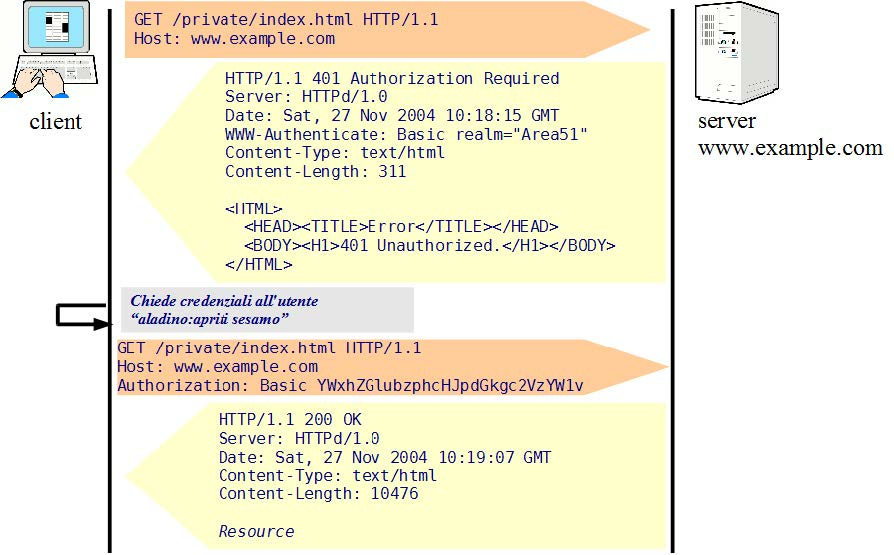
\includegraphics[width=\linewidth]{Images/Basic_access_authentication.jpg}
	\caption{Example of basic access authentication}
	\label{fig:basic_authentication}
\end{figure}

Basic access authentication is the simplest HTTP authentication scheme. The server challenge specifies the scheme \texttt{Basic} and the realm name. The user agent asks the user for a username and password, combines them into a single credential string, encodes the result with Base64, and sends it in the \texttt{Authorization} header field.

\begin{lstlisting}
HTTP/1.1 401 Unauthorized
WWW-Authenticate: Basic realm="Restricted area"

GET /private/index.html HTTP/1.1
Host: www.example.org
Authorization: Basic base64(username:password)
\end{lstlisting}

The value sent after \texttt{Basic} is only encoded, not encrypted. Base64 is a reversible textual representation of bytes; it does not provide confidentiality. Consequently, Basic authentication exposes the password to any entity able to observe the traffic unless the HTTP exchange is protected by a secure transport layer.\\

The weakness of Basic authentication is therefore not the use of a realm or the challenge-response structure, but the fact that the reusable secret is transmitted in a trivially decodable form. Its use is acceptable only when another mechanism protects the communication channel.

\subsection{Digest Access Authentication}

\begin{figure}[!h]
	\centering
	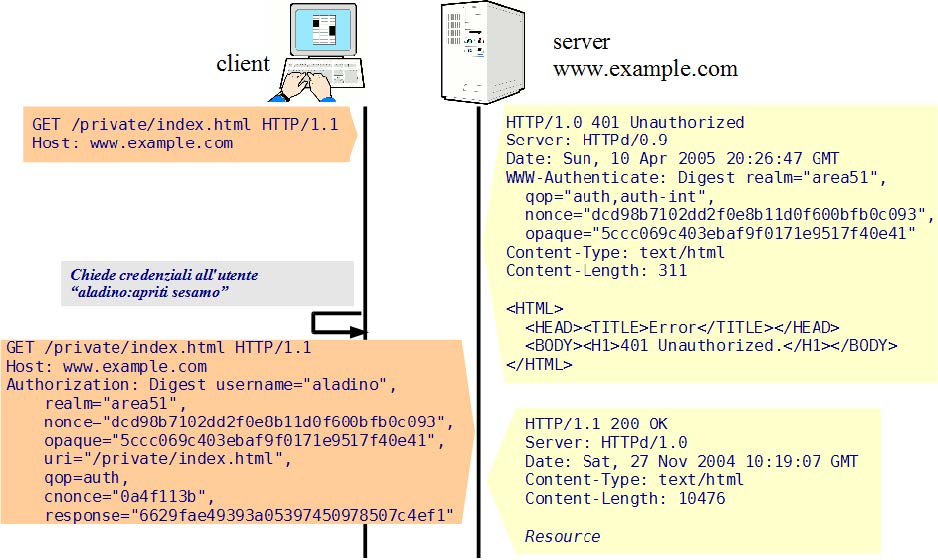
\includegraphics[width=\linewidth]{Images/Digest_access_authentication.jpg}
	\caption{Example of digest access authentication}
	\label{fig:digest_authentication}
\end{figure}

Digest access authentication improves the previous scheme by avoiding the direct transmission of the password. Instead of sending the password itself, the client sends a digest value computed from the password and from challenge data supplied by the server. The classical formulation uses the \texttt{MD5} (Message Digest 5) hash function.\\

The server challenge specifies the \texttt{Digest} scheme and includes parameters such as the realm, a nonce, an opaque value, and possibly a quality-of-protection parameter.

\begin{lstlisting}
HTTP/1.1 401 Unauthorized
WWW-Authenticate: Digest realm="Restricted area",
                  qop="auth,auth-int",
                  nonce="server-generated-nonce",
                  opaque="server-generated-opaque-value"
\end{lstlisting}

The \texttt{nonce} is a value generated by the server, typically changing across challenges. It prevents a captured authentication response from being reused directly in a later exchange. The \texttt{opaque} value is an additional server-generated string that the client must return unchanged. The quality-of-protection parameter can require additional data to be included in the computation.\\

In the basic case where no additional quality-of-protection mechanism is considered, the client computes the fingerprint using the username, realm, password, request method, requested URI, and server nonce.

\begin{lstlisting}
h1       = MD5(username:realm:password)
h2       = MD5(method:digestURI)
response = MD5(h1:nonce:h2)
\end{lstlisting}

The subsequent request contains the authentication parameters and the computed response.

\begin{lstlisting}
GET /private/index.html HTTP/1.1
Host: www.example.org
Authorization: Digest username="alice",
                      realm="Restricted area",
                      nonce="server-generated-nonce",
                      uri="/private/index.html",
                      qop=auth,
                      nc=00000001,
                      cnonce="client-generated-nonce",
                      response="computed-digest",
                      opaque="server-generated-opaque-value"
\end{lstlisting}

The server can verify the request because it knows the expected password or an equivalent secret associated with the username. It recomputes the same digest from the received parameters and compares it with the \texttt{response} value provided by the client. If the values match, the server authorizes the request.\\

Digest authentication mitigates the most evident flaw of Basic authentication because the password is not sent in clear text. However, it does not make the communication channel confidential. The request URI, headers, and response content may still be visible to observers unless the connection is protected separately. Digest authentication should therefore be understood as an authentication mechanism, not as a complete security model for HTTP communication.

\subsection{Creation of Realms in Web Server Configuration}

A \textbf{realm} is not a physical directory by itself. It is a protection space associated with one or more resources and identified by a textual name sent to the client in the authentication challenge. The same realm name may protect several URI spaces, and different realms may be defined even inside the same web application. From the point of view of the user agent, the realm helps determine when previously supplied credentials can be reused.\\

In a practical server configuration, creating a realm usually means associating an authentication scheme, a realm name, a credential source, and an authorization rule with a directory, location, or URI prefix. The web server then automatically performs the HTTP challenge-response exchange when a request targets a protected resource.\\

For example, in Apache HTTP Server, Basic authentication for a directory can be configured as follows:

\begin{lstlisting}
<Directory "/var/www/html/private">
  AuthType Basic
  AuthName "Restricted Area"
  AuthUserFile "/etc/apache2/.htpasswd"
  Require valid-user
</Directory>
\end{lstlisting}

The directive \texttt{AuthType Basic} selects the Basic authentication scheme. The directive \texttt{AuthName} defines the realm name, which appears in the \texttt{WWW-Authenticate} challenge. The directive \texttt{AuthUserFile} specifies the file containing the allowed users and password hashes. Finally, \texttt{Require valid-user} states that any authenticated user listed in the credential file is allowed to access the protected resources.\\

A similar protection space can also be configured through a local \texttt{.htaccess} file when the server configuration permits it. The \texttt{.htaccess} file contains the access-control directives, while the credential file referenced by \texttt{AuthUserFile} contains the valid usernames and password hashes. For example, a \texttt{.htaccess} file placed inside a protected directory may contain:

\begin{lstlisting}
AuthType Basic
AuthName "Restricted Area"
AuthUserFile "/etc/apache2/.htpasswd"
Require valid-user
\end{lstlisting}

In this case, the directory structure is used as a convenient way to associate the protection rule with a set of resources. However, the realm is still the logical protection space named by \texttt{AuthName}, not the directory itself. The file referenced by \texttt{AuthUserFile} is not the local configuration file; it is the credential store used by Apache to verify the supplied username and password.\\

In NGINX, the same idea is commonly expressed inside a \texttt{location} block:

\begin{lstlisting}
location /private/ {
  auth_basic "Restricted Area";
  auth_basic_user_file /etc/nginx/.htpasswd;
}
\end{lstlisting}

The directive \texttt{auth\_basic} enables Basic authentication and defines the realm string. The directive \texttt{auth\_basic\_user\_file} specifies the file containing the valid credentials. Requests whose URI starts with \texttt{/private/} are therefore challenged before the resource is served or before the request is forwarded to an upstream application.\\

The creation of a realm can therefore be understood as a server-side binding:

\begin{lstlisting}
protected URI space
+ authentication scheme
+ realm name
+ credential source
+ authorization rule
\end{lstlisting}

The client does not create the realm. The server defines it and advertises it through \texttt{WWW-Authenticate} when access to a protected resource requires credentials.

\subsection{HTTP Authentication and Application-Level Authentication}

HTTP authentication and application-level authentication solve related but distinct problems. HTTP authentication is part of the protocol. It is based on response and request headers such as \texttt{WWW-Authenticate} and \texttt{Authorization}. Application-level authentication is instead implemented by server-side code, such as PHP, Java, Python, or a backend framework. In that case, HTTP only transports the form fields, JSON objects, cookies, or tokens used by the application.\\

With HTTP Basic authentication, the browser reacts to a \texttt{401 Unauthorized} response containing a challenge such as:

\begin{lstlisting}
HTTP/1.1 401 Unauthorized
WWW-Authenticate: Basic realm="Restricted Area"
\end{lstlisting}

The browser then sends a new request containing an \texttt{Authorization} header:

\begin{lstlisting}
GET /private/index.html HTTP/1.1
Host: www.example.org
Authorization: Basic YWxpY2U6c2VjcmV0
\end{lstlisting}

The value after \texttt{Basic} is a Base64 representation of the pair \texttt{username:password}. Base64 is an encoding, not a cryptographic protection. For this reason, Basic authentication must be used only over a protected transport channel, such as HTTPS, whenever credentials have to be kept confidential.\\

With HTTP Digest authentication, the password is not sent directly. The server sends a challenge containing parameters such as the realm, a nonce, and the selected algorithm. The client computes a digest using information including the username, password, realm, nonce, HTTP method, and requested URI. The resulting value is sent in the \texttt{Authorization} header. The server can verify the response by performing the corresponding computation on its side.\\

This mechanism is different from a PHP login form. In an application-level login, the browser usually sends credentials as normal request data:

\begin{lstlisting}
POST /login.php HTTP/1.1
Host: www.example.org
Content-Type: application/x-www-form-urlencoded

username=alice&password=secret
\end{lstlisting}

The web server passes the request to the PHP application. PHP reads the submitted fields, queries the user database, verifies the password, and, if authentication succeeds, creates an application session or returns an application token. The HTTP protocol does not automatically know that the field named \texttt{password} contains a password, nor does it know whether the application will hash it, compare it, reject it, or ignore it.\\

For this reason, if a PHP script computes a value such as:

\begin{lstlisting}
$hash = md5($_POST["password"]);
\end{lstlisting}

the server does not know this because of HTTP. It happens because the application code explicitly performs that operation. The client and server share the meaning of the submitted data only according to the application protocol implemented above HTTP. Moreover, MD5 should not be used for password storage in modern applications. Passwords should be stored using password-hashing mechanisms designed for that purpose, for example through functions such as \texttt{password\_hash()} and verified through \texttt{password\_verify()} in PHP.\\

The essential distinction is therefore:

\begin{itemize}
	\item in \textbf{HTTP authentication}, the authentication scheme is negotiated at the HTTP level through standard headers;
	\item in \textbf{application-level authentication}, the authentication procedure is defined by the application and merely transported by HTTP messages.
\end{itemize}

The two mechanisms may also coexist. For example, a reverse proxy or web server may require HTTP Basic authentication before allowing access to an internal administrative area, while the application behind it still performs its own login and authorization checks. In such a configuration, HTTP authentication protects the entry point, whereas the application decides what the authenticated user is allowed to do inside the system.

\subsection{Comparison Between HTTP Authentication and Application-Level Authentication}

HTTP authentication is simple, standardized, and directly supported by browsers, web servers, and proxies. It is suitable when the access-control model is coarse-grained: a directory, URI prefix, internal tool, staging environment, documentation area, or simple API endpoint must be protected by a relatively small set of credentials. Since the web server can enforce the check before the application is invoked, HTTP authentication can also reduce the amount of application code needed for simple protected resources.\\

Its limitations appear when the authentication and authorization model becomes application-specific. HTTP Basic and Digest are centered on credentials for a realm; they do not directly provide a customizable login page, password reset workflow, registration process, multi-factor authentication, user profile management, fine-grained roles, per-object permissions, or application-specific session logic. Browser support is also rigid: the standard Basic authentication dialog is controlled by the user agent and is not designed as a full application login interface.\\

Application-level authentication is more flexible. It allows the application to define its own login pages, credential policies, database schema, sessions, cookies, tokens, roles, permissions, audit logs, and user experience. It is the usual choice for web applications where authentication is part of the domain logic. For example, an e-commerce platform, a social network, a learning management system, or an administrative dashboard usually needs to distinguish not only between authenticated and unauthenticated users, but also between users with different privileges and different relationships to specific resources.\\

The trade-off is that application-level authentication requires more implementation care. The application must correctly handle password hashing, session generation, cookie security, logout, expiration, authorization checks, rate limiting, protection against common web attacks, and integration with external identity providers when needed. HTTP carries the messages, but the application remains responsible for the security semantics.

\begin{center}
	\begin{tabularx}{\linewidth}{p{0.21\textwidth}p{0.3\textwidth}X}
		\textbf{Aspect} & \textbf{HTTP authentication} & \textbf{Application-level authentication} \\
		\hline
		Main layer & Protocol and server/proxy configuration & Application logic \\ \hline
		
		Typical mechanism & \texttt{WWW-Authenticate} and \texttt{Authorization} headers & Forms, JSON requests, cookies, sessions, tokens \\ \hline
		
		Configuration point & Web server, reverse proxy, API gateway & Backend application or authentication service \\ \hline
		
		Granularity & Realm, directory, location, URI prefix & User roles, object permissions, business rules \\ \hline
		
		User interface & Browser-controlled or client-controlled & Fully customizable \\ \hline
		
		Best suited for & Internal tools, protected directories, simple APIs, staging areas & Full web applications, user accounts, complex authorization \\ \hline
		
		Main limitation & Limited flexibility and weak user experience & Requires careful secure implementation \\ \hline
	\end{tabularx}
\end{center}

A practical rule is the following. Use HTTP authentication when the protected area is simple and the authorization rule is mostly independent of application data. Use application-level authentication when identity, roles, sessions, and permissions are part of the application semantics. Use both when a coarse-grained external barrier is useful in addition to fine-grained application checks, for example when an internal administration interface is protected by a reverse proxy and the application still verifies the privileges of each logged-in user.

\section{HTTP Connections}

\begin{figure}[!h]
	\centering
	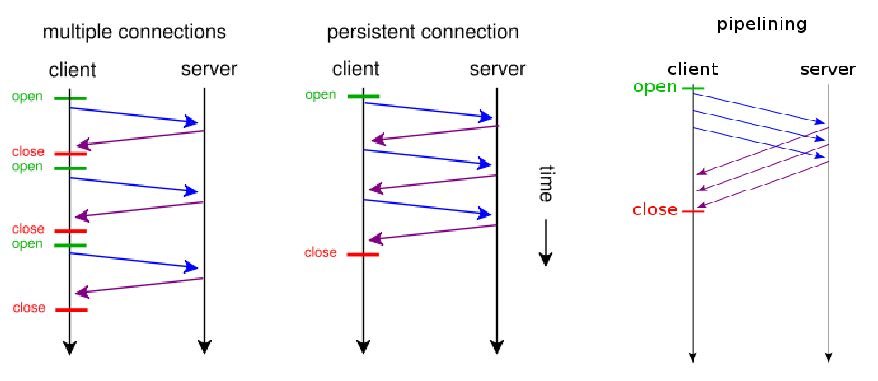
\includegraphics[width=\linewidth]{Images/HTTP_connections.jpg}
	\caption{The three types of HTTP connection}
	\label{fig:http_connections}
\end{figure}

An HTTP connection is the transport context in which a sequence of HTTP requests and corresponding HTTP responses is exchanged. Since HTTP relies on TCP in the classical Web stack, a TCP connection must exist before the HTTP messages can be transmitted.\\

A naive strategy would open a separate TCP connection for every request-response pair. This is simple, but expensive. Each connection requires setup and teardown, and both endpoints must maintain state for the open connection. The overhead becomes significant because a single Web page usually depends on several resources: the main HTML document, style sheets, scripts, images, and other linked objects.\\

Connection management therefore aims to reuse the same transport connection when this reduces latency and avoids unnecessary setup costs.

\subsection{Persistent Connections}

A persistent connection allows multiple request-response exchanges to use the same TCP connection. The connection remains open after one response so that the client can issue further requests without repeating the TCP setup phase.\\

In HTTP/1.0, connections are not persistent by default. A client can request persistence by using the \texttt{Connection} header field with the value \texttt{Keep-Alive}. If the server supports persistent connections, it includes the same indication in its response.

\begin{lstlisting}
GET /index.html HTTP/1.0
Host: www.example.org
Connection: Keep-Alive

HTTP/1.0 200 OK
Connection: Keep-Alive
Content-Type: text/html
Content-Length: 1250
\end{lstlisting}

In HTTP/1.1, persistent connections are the default behavior. If the server decides to close the connection after the response, it explicitly signals this decision with \texttt{Connection: close}.

\begin{lstlisting}
HTTP/1.1 200 OK
Connection: close
Content-Type: text/html
Content-Length: 1250
\end{lstlisting}

Persistent connections improve the utilization of the underlying TCP connection, but they cannot remain open indefinitely. Both clients and servers use timeouts to close connections that remain inactive for too long. This prevents idle connections from consuming resources without contributing to useful communication.

\newpage
\subsection{Pipelining}

Pipelining is the transmission of multiple requests on a persistent connection without waiting for the complete response to a previous request. The client can send a sequence of requests to the same server, and the server later returns the corresponding responses.

\begin{lstlisting}
GET /index.html HTTP/1.1
Host: www.example.org

GET /style.css HTTP/1.1
Host: www.example.org

GET /logo.png HTTP/1.1
Host: www.example.org
\end{lstlisting}

Pipelining reduces latency because it avoids idle time between consecutive requests. This is relevant for Web pages composed of resources with different sizes or different server-side processing costs.\\

The ordering constraint is fundamental. HTTP does not include an explicit response identifier that binds each response to a specific earlier request. Therefore, responses must be sent in the same order in which the corresponding requests were received. The client reconstructs the association between requests and responses from this ordering.\\

This mechanism optimizes traffic in common browsing scenarios, but it also exposes a limitation of ordered response delivery: a slow first response can delay later responses even when the corresponding resources are ready earlier.

\section{Session Management over a Stateless Protocol}

HTTP is stateless: a request is processed as an independent interaction, and the protocol does not require the server to remember previous requests from the same client. This property simplifies the protocol and reduces mandatory coupling between interactions, but it is not sufficient for many Web applications.\\

A transaction or user session often spans several requests. Examples include authentication flows, shopping carts, multi-step forms, and personalized application areas. In these cases, the server must associate the current request with a previous context. Since this association is not provided by HTTP itself, it must be reconstructed through additional mechanisms.\\

It is important to distinguish session management from persistent connections. A persistent connection reuses a transport channel; a session reconstructs application-level continuity. A user session may continue across several TCP connections, and a persistent connection does not by itself identify the user or the application transaction.

\newpage
\subsection{Cookies}

\begin{figure}[!h]
	\centering
	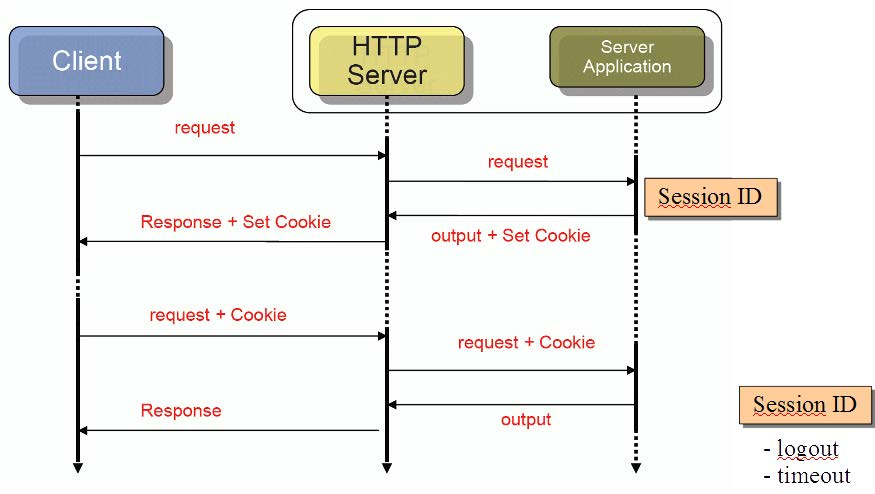
\includegraphics[width=\linewidth]{Images/Cookie.jpg}
	\caption{Example of cookie-based session management. The server creates client-side state by sending a cookie in the first response; the browser then includes that cookie in subsequent requests, allowing the server to associate them with the same session. The final exchange illustrates cookie invalidation, either after an explicit logout or after session expiration due to inactivity.}
	\label{fig:cookie}
\end{figure}

A cookie (or magic cookie) is a small opaque piece of information exchanged between the server and the user agent. It is opaque because the client is not expected to interpret its internal structure. The value is meaningful primarily to the server, which can associate it with an application session, a transaction, or a user profile.\\

The server creates a cookie by sending the \texttt{Set-Cookie} header in a response. The user agent may store the value locally and send it back in subsequent requests using the \texttt{Cookie} header (see figure \ref{fig:cookie}). The decision to send a stored cookie is based on attributes such as the target server, the resource URL, and the cookie lifetime.

\begin{lstlisting}
HTTP/1.1 200 OK
Content-Type: text/html
Set-Cookie: SID=31d4d96e407aad42; Path=/; Max-Age=3600

GET /cart HTTP/1.1
Host: shop.example.org
Cookie: SID=31d4d96e407aad42
\end{lstlisting}

A typical architecture separates the HTTP server from the application logic. The application server creates a new session identifier and associates it with internal state. The HTTP response carries that identifier as a cookie. On a later request, the browser returns the cookie, and the server-side application uses the identifier to recover the corresponding session state.\\

The cookie value can expire. Expiration may be explicit, through attributes such as a maximum age, or implicit, for example when the user logs out or when the server invalidates the session after inactivity.\\

Cookies are widely used because they solve a precise problem with limited protocol machinery: they allow a stateless request-response protocol to support application-level continuity. They are also flexible enough to support authentication sessions, multi-step transactions, and personalization.

\subsection{Alternatives to Cookies}

Other mechanisms can be used to associate requests with previous state, but each introduces practical drawbacks.\\

A first possibility is to associate the state with the requester IP address. This is unreliable because several users may share the same address, for example behind a proxy or a network address translator, while a single user may obtain different addresses across time.\\

A second possibility is to store state information inside dynamically generated HTML pages, for instance in hidden form fields. This makes the state page-specific, requires dynamic generation of the relevant pages, and exposes the state value to simple client-side manipulation unless additional protection is added.\\

A third possibility is to encode state directly inside URLs. This complicates interaction with proxies and caches, makes the state visible in logs and shared links, and increases the risk that the opaque value is manipulated or leaked.\\

Cookies became the dominant mechanism because they provide a compact and general way to reconnect requests with server-side context without modifying every URL or every page body.

\subsection{First-Party and Third-Party Cookies}

From a security and privacy perspective, a relevant distinction is between first-party and third-party cookies.\\

A first-party cookie is associated with the site that the user is directly visiting. It is commonly used for sessions, transactions, access continuity, and site-specific personalization. Although it still requires careful handling, its role is directly connected to the requested service.\\

A third-party cookie is associated with a domain different from the one displayed to the user. This occurs when a page includes resources from external providers, such as advertisements, tracking pixels, or embedded social components. The browser may contact the external domain while rendering the page, and that external domain may set or receive its own cookie.\\

This mechanism allows the same external provider to recognize a user across several unrelated sites that embed resources from that provider. It is therefore useful for cross-site profiling and advertising networks, but it has significant privacy implications because the tracking is not necessarily visible in the main address shown to the user.

\begin{lstlisting}
GET /news/article.html HTTP/1.1
Host: news.example.org

GET /banner.png HTTP/1.1
Host: ads.example.net
Cookie: ADID=external-provider-cookie
\end{lstlisting}

The technical mechanism is the same as for ordinary cookies: \texttt{Set-Cookie} in a response and \texttt{Cookie} in later requests. The difference lies in the relationship between the resource requested by the user and the domain receiving the cookie.\\

A proposed convention for reducing this kind of tracking is the \texttt{DNT} (Do Not Track) header field. When enabled by the user agent, it expresses that the user does not want to be tracked.

\begin{lstlisting}
DNT: 1
\end{lstlisting}

This indication is a request for behavior by the receiving server; it is not, by itself, a cryptographic or protocol-level enforcement mechanism. The privacy properties of cookie-based systems therefore depend not only on HTTP syntax, but also on browser policies, server behavior, and the surrounding application architecture.

\chapter{Proxy Servers and HTTP Caching}

\section{Proxy Servers}

\begin{figure}[!h]
	\centering
	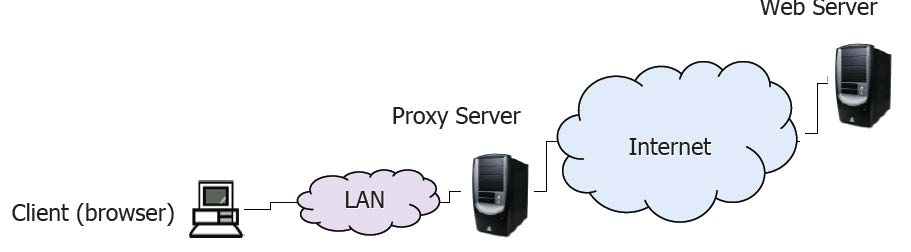
\includegraphics[width=\linewidth]{Images/Proxy_server.jpg}
	\caption{Example of client server interaction with a proxy server acting as an intermediary.}
	\label{fig:proxy}
\end{figure}

A proxy server is an intermediary application placed between clients and origin servers (see figure \ref{fig:proxy}). From the client-side perspective, the proxy receives HTTP requests and determines whether it can answer them directly, whether it should forward them to another server, or whether it should reject them according to local policy. From the server-side perspective, the proxy behaves as a client when it forwards requests toward the origin server.\\

The proxy role is therefore not limited to simple forwarding. A proxy can inspect requests and responses, apply access-control rules, store reusable responses, and transform or adapt the communication when this is permitted by the protocol and by the deployment architecture.

\subsection{Proxy Cache}

A common use of a proxy is caching. When several clients request the same URL, or when the same client repeatedly requests it, the proxy can store a response obtained from the origin server and reuse it later. If the stored response is still valid, the proxy sends it directly to the client, avoiding a new request to the origin server.\\

This is particularly effective when the proxy is located close to the clients, for example at the border of a local area network. In that case, a cache hit reduces both latency and external network traffic. A cache miss, instead, forces the proxy to contact the origin server and therefore provides no immediate bandwidth saving for that request. The usefulness of a proxy cache depends strongly on the ratio between hits and misses, on the validity lifetime of stored resources, and on the cost of validating possibly stale entries.

\newpage
\begin{lstlisting}
Client                  Proxy cache             Origin server
  | GET /logo.png           |                         |
  |------------------------>|                         |
  |                         | GET /logo.png           |
  |                         |------------------------>|
  |                         | 200 OK + representation |
  |                         |<------------------------|
  | 200 OK + representation |                         |
  |<------------------------|                         |
\end{lstlisting}

Later request, cache hit:

\begin{lstlisting}
Client                        Proxy cache             Origin server
  | GET /logo.png                 |                         |
  |------------------------------>|                         |
  |                               |                         |
  | 200 OK + cached representation|                         |
  |<------------------------------|                         |
\end{lstlisting}

A proxy cache is not a mirror of the origin server. It can answer only when it already owns a reusable representation and the cache metadata allows reuse. Otherwise, it must behave as a client toward the origin server, obtain or validate the resource, and only then answer the requesting client.

\subsection{Proxy Filtering}

A proxy can also act as a filter. In this configuration, requests are forwarded only when they satisfy the network security and control policy. This is common in managed networks, where access to external domains, IP addresses, or resource categories may be restricted.\\

Two basic filtering strategies are commonly used. A blacklist denies access to explicitly prohibited destinations and allows the rest. A whitelist allows access only to explicitly admitted destinations and denies all the others. If a request violates the policy, the proxy does not forward it to the origin server and returns an authorization or access-control failure response to the client.

\section{Reverse Proxies}

\begin{figure}[!h]
	\centering
	\includegraphics[width=\linewidth]{Images/Reverse\_proxy.jpg}
	\caption{Figure showing that the reverse proxy acts as a gateway for the internal network containing one or more origin servers.}
	\label{fig:reverse_proxy}
\end{figure}

A reverse proxy is a proxy server placed in front of one or more Web servers. The client contacts the reverse proxy as if it were the origin server, while the reverse proxy forwards the request to an internal server that actually hosts or generates the requested resource (see figure \ref{fig:reverse_proxy}).\\

The term \emph{reverse} emphasizes that the proxy protects and organizes the server side rather than representing a set of clients. A forward proxy is typically introduced by or for clients; a reverse proxy is introduced by the service provider and is part of the server-side architecture.

\subsection{Main Objectives}

A reverse proxy enables several architectural functions.\\

First, it allows multiple Web servers to share a single public address and a single public entry point. The reverse proxy receives the external requests and dispatches them to the appropriate internal server according to host name, path, application, or load-balancing policy.\\

Second, it supports load balancing. When a service is replicated across several server instances, the reverse proxy can distribute incoming requests among them. This enables scale-out: instead of increasing the capacity of a single machine indefinitely, the service provider adds several machines and distributes the work across them.\\

Third, it can enforce a firewall-like separation between the public Internet and the internal server network. The origin servers do not need to be directly exposed to clients. The reverse proxy becomes the controlled contact point where request filtering, logging, rate limiting, and routing decisions can be centralized.\\

Fourth, it can cache responses. This reduces the load on the internal servers when many clients request the same reusable resources.\\

Finally, a reverse proxy can perform hardware-accelerated cryptographic operations for secure connections. In such deployments, the external connection is protected, while the reverse proxy centralizes expensive cryptographic processing, certificate handling, and security policy enforcement. The precise security properties depend on whether the internal segment between the reverse proxy and the origin servers is also protected.

\section{HTTP Caching}

Caching is the technique of storing a previously obtained response so that it can be reused for later requests. Its goals are to reduce latency, reduce network overhead, and reduce repeated processing at the origin server.\\

HTTP caching can be placed in different positions:

\begin{itemize}
    \item a \textbf{client-side cache}, usually controlled by the user agent;
    \item a \textbf{server-side cache}, located near or inside the server infrastructure;
    \item an \textbf{intermediate cache}, typically implemented by a proxy.
\end{itemize}

A server-side cache can reduce response generation time, but the response still has to cross the network to reach the client. Client-side and proxy caches can also reduce network load, because a valid stored representation can be reused without retrieving the full resource again from the origin server.\\

The central problem of caching is not only storing responses, but deciding whether a stored response is still acceptable. HTTP therefore provides mechanisms for freshness, expiration, and validation.

\section{Cache Control in Early HTTP}

HTTP/1.0 used a small set of header fields to support basic cache management.

\subsection{The \texttt{Expires} Header}

The \texttt{Expires} header allows the server to attach an absolute expiration date to the response. Until that date, a cache may consider the response fresh. After that date, the response is stale and must be revalidated before ordinary reuse.

\begin{lstlisting}
HTTP/1.0 200 OK
Date: Tue, 03 Jun 2026 10:00:00 GMT
Expires: Tue, 03 Jun 2026 12:00:00 GMT
Content-Type: text/html
Content-Length: 1250
\end{lstlisting}

This mechanism requires the interpretation of timestamps. It therefore assumes that the systems involved have reasonably consistent clocks. HTTP does not define how clock synchronization is achieved; it only defines how the timestamps are carried and interpreted.

\subsection{The \texttt{Pragma: no-cache} Header}

The \texttt{Pragma: no-cache} header was used to indicate that a response should not be reused from cache without contacting the origin server. It is a legacy mechanism and is less expressive than the later \texttt{Cache-Control} directives, but it captures an important requirement: not all resources are suitable for caching. Dynamically generated pages, personalized responses, and transaction-related representations often require stricter cache behavior.

\subsection{The \texttt{If-Modified-Since} Header}

The \texttt{If-Modified-Since} header allows a client or cache to make a conditional request. The request asks the server to send the representation only if the resource has changed after the specified date.

\begin{lstlisting}
GET /index.html HTTP/1.0
Host: www.example.org
If-Modified-Since: Tue, 03 Jun 2026 10:00:00 GMT
\end{lstlisting}

If the resource has changed, the server returns the new representation. If it has not changed, the server can return a response without the body, typically using \texttt{304 Not Modified}. This avoids retransmitting an unchanged resource.

\section{Server-Specified Expiration}

HTTP/1.1 provides more structured cache control. In server-specified expiration, the origin server determines the freshness lifetime of the response. This can be done with the older \texttt{Expires} header or with the \texttt{max-age} directive in \texttt{Cache-Control}.

\begin{lstlisting}
HTTP/1.1 200 OK
Date: Tue, 03 Jun 2026 10:00:00 GMT
Cache-Control: max-age=3600
Content-Type: text/css
Content-Length: 8400
\end{lstlisting}

In this example, the response is fresh for 3600 seconds from the response date. During that interval, a cache may reuse the response without contacting the origin server, unless another directive or request condition prevents it.

\subsection{Fresh and Stale Responses}

A cached response is \emph{fresh} while its freshness lifetime has not expired. After that, it is \emph{stale}. A stale response normally has to be revalidated before it can be used as an ordinary response.\\

In some situations, a cache may serve a stale response. For example, a client may be willing to accept an expired response, or the origin server may temporarily be unreachable. When a stale response is returned, the response should indicate that the representation is stale. The warning code \texttt{110 Response is stale} is used for this purpose.

\begin{lstlisting}
HTTP/1.1 200 OK
Date: Tue, 03 Jun 2026 12:05:00 GMT
Warning: 110 - "Response is stale"
Content-Type: text/html
Content-Length: 1250
\end{lstlisting}

Serving stale content is a trade-off: it may improve availability and latency, but it can also expose the client to an outdated representation.

\subsection{The \texttt{must-revalidate} Directive}

The \texttt{must-revalidate} directive prevents a cache from returning a stale response without successful validation. Once the response has expired, the cache must contact the origin server and verify whether the representation is still valid.

\begin{lstlisting}
Cache-Control: max-age=600, must-revalidate
\end{lstlisting}

If the cached response is stale and the origin server cannot be reached, the cache must not answer with the expired representation. In that case, it should return an error such as \texttt{504 Gateway Timeout}.

\subsection{The \texttt{no-cache} Directive}

Despite its name, \texttt{no-cache} does not necessarily mean that the response cannot be stored. It means that the stored response must not be reused to satisfy a later request without validation with the origin server. The cache may keep the representation, but each reuse requires a successful check.

\begin{lstlisting}
Cache-Control: no-cache
\end{lstlisting}

This directive is useful when storage is acceptable but freshness must be verified before every use.

\section{Heuristic Expiration}

Not all responses include explicit freshness information. When neither \texttt{Expires} nor suitable \texttt{Cache-Control} directives are available, a cache may estimate a freshness lifetime heuristically.\\

A common heuristic is based on the time elapsed since the resource was last modified. The idea is that a resource that has remained unchanged for a long time is likely to remain unchanged for a short additional interval.

\begin{lstlisting}
expiry-period = time-since-last-modified-date * factor
expiry-date   = current-date + expiry-period

typical factor = 0.1
\end{lstlisting}

For example, if a resource has not changed for 10 hours and the factor is \texttt{0.1}, the cache may consider it fresh for approximately one additional hour.\\

Heuristic expiration is necessarily uncertain. It may be conservative in many cases, but it can also be optimistic: the resource may change before the estimated expiration date. When a cache uses a heuristic freshness lifetime and the response is old enough for the heuristic to be questionable, it can include the warning code \texttt{113 Heuristic expiration}.

\begin{lstlisting}
HTTP/1.1 200 OK
Warning: 113 - "Heuristic expiration"
Content-Type: image/png
Content-Length: 48210
\end{lstlisting}

The warning does not invalidate the response by itself. It informs the client that the freshness decision was derived from a heuristic rather than from explicit server-provided expiration metadata.

\section{Cache Validation}

Expiration determines when a cached response becomes stale. Validation determines whether a stale response can still be used because the origin resource has not changed.\\

In many cases, a response becomes stale even though the resource on the origin server is unchanged. Re-downloading the full representation would be wasteful. HTTP validation mechanisms allow a cache to check whether its stored representation is still current while avoiding unnecessary transfer of the body.

\subsection{Validation with \texttt{HEAD}}

A simple validation strategy is to send a \texttt{HEAD} request for the resource. The server returns the header section that would accompany a \texttt{GET} response, but without the body. The cache can compare metadata such as \texttt{Last-Modified}, \texttt{Content-Length}, or validators with its stored entry.

\begin{lstlisting}
HEAD /manual.pdf HTTP/1.1
Host: www.example.org

HTTP/1.1 200 OK
Last-Modified: Tue, 03 Jun 2026 09:15:00 GMT
Content-Length: 245760
Content-Type: application/pdf
\end{lstlisting}

This reduces the cost of validation because the body is not transmitted. However, it introduces an additional request-response exchange. If the resource is found to be outdated, the cache must still send a later \texttt{GET} request to retrieve the new representation.

\subsection{Conditional Requests}

A more efficient strategy is to make the retrieval itself conditional. The client or cache sends a \texttt{GET} request with a condition. If the condition shows that the stored representation is still valid, the server returns \texttt{304 Not Modified} without a body. If the resource has changed, the server returns the new representation in the ordinary response.

\begin{lstlisting}
GET /manual.pdf HTTP/1.1
Host: www.example.org
If-Modified-Since: Tue, 03 Jun 2026 09:15:00 GMT

HTTP/1.1 304 Not Modified
Date: Tue, 03 Jun 2026 11:00:00 GMT
\end{lstlisting}

This approach reduces both the number of requests and the number of full body transfers compared with a preliminary \texttt{HEAD} request followed by a possible \texttt{GET}.

\section{Validators and Entity Tags}

A validator is metadata that identifies a specific version of a resource representation. Entity tags, carried by the \texttt{ETag} header field, are a central validation mechanism in HTTP. When the origin server returns a representation, it may attach an entity tag to that representation.

\begin{lstlisting}
HTTP/1.1 200 OK
Date: Tue, 03 Jun 2026 10:00:00 GMT
ETag: "a9f37c12"
Content-Type: text/html
Content-Length: 1250
\end{lstlisting}

The cache stores the entity tag together with the response. Later, it can use that tag in a conditional request to determine whether the representation it owns still matches the current representation at the origin server.

\subsection{Strong and Weak Validators}

A strong validator changes whenever the representation changes at the binary level. It is suitable when byte-for-byte equality matters, for example for range requests or exact cache validation.\\

A weak validator expresses semantic equivalence rather than binary equality. It may remain unchanged across modifications that do not alter the meaningful content of the resource. Weak entity tags are marked with the \texttt{W/} prefix.

\begin{lstlisting}
ETag: "strong-validator-value"
ETag: W/"weak-validator-value"
\end{lstlisting}

The choice between strong and weak validators is made by the server. Strong validators provide stricter guarantees; weak validators allow the server to treat several binary representations as equivalent when the application semantics justify it.

\subsection{The \texttt{If-None-Match} Header}

The \texttt{If-None-Match} header makes the request conditional on the absence of a match between the entity tags supplied by the client and the current entity tag of the resource.\\

For \texttt{GET} and \texttt{HEAD}, this is typically used for cache validation. If none of the supplied tags matches the current entity tag, the server executes the method and sends the current representation. If there is a match, the cached representation is still current and the server returns \texttt{304 Not Modified}.

\begin{lstlisting}
GET /index.html HTTP/1.1
Host: www.example.org
If-None-Match: "a9f37c12"

HTTP/1.1 304 Not Modified
Date: Tue, 03 Jun 2026 11:00:00 GMT
ETag: "a9f37c12"
\end{lstlisting}

For methods other than \texttt{GET} and \texttt{HEAD}, a match causes the request not to be executed and the server returns \texttt{412 Precondition Failed}. This prevents an operation from being applied under a precondition that is no longer satisfied.

\subsection{The \texttt{If-Match} Header}

The \texttt{If-Match} header has the opposite condition. The method is executed only if at least one entity tag provided by the client matches the current entity tag of the resource. If no tag matches, the server returns \texttt{412 Precondition Failed}.

\begin{lstlisting}
PUT /document.txt HTTP/1.1
Host: www.example.org
If-Match: "a9f37c12"
Content-Type: text/plain
Content-Length: 21

Updated document text.

HTTP/1.1 412 Precondition Failed
Date: Tue, 03 Jun 2026 11:00:00 GMT
\end{lstlisting}

This mechanism is important for update operations. A client can avoid overwriting a resource that has been changed by someone else after the client obtained its local copy. The entity tag then acts as a compact representation-version identifier, allowing HTTP to support consistency checks without introducing server-side session state.

\section{Caching as a Consistency Trade-Off}

HTTP caching improves performance by reusing representations, but every cache introduces a consistency problem: the cache may own a representation that is no longer identical to the origin resource. Expiration policies reduce the need for validation during a freshness interval; validation mechanisms reduce the cost of checking stale entries; entity tags provide precise representation-version metadata.\\

The main engineering decision is therefore not whether caching is useful, but how aggressive it should be. Static resources with stable content can use long freshness lifetimes. Dynamic, personalized, or transaction-sensitive resources require strict validation or avoidance of reuse. Proxy caches are effective when many users share requests for the same resources, while client caches are effective for repeated access by the same user agent. Reverse proxies use caching mainly to protect and accelerate the server side.\\

Correct cache design combines these mechanisms: explicit server directives when the origin server knows the validity policy, heuristic expiration only when explicit metadata is absent, and conditional validation whenever a stale resource might still be reusable.

\chapter{Security Models for HTTP}

\section{Security Requirements in HTTP Communication}

HTTP was originally designed as a simple application-layer protocol for exchanging resources through a request--response interaction. In its basic form, the protocol does not provide confidentiality, integrity protection, or endpoint authentication. A request message and the corresponding response can therefore be inspected or modified by any entity that is able to observe or interfere with the communication path.\\

Secure HTTP communication must address three main requirements:
\begin{enumerate}
	\item \textbf{Confidentiality} prevents unauthorized entities from reading the exchanged content;
	\item \textbf{Integrity} allows the communicating parties to detect modifications of messages during transmission;
	\item \textbf{Authentication} allows a party to verify the identity of the peer, most commonly the server contacted by the client.
\end{enumerate}

These requirements are independent from the ordinary HTTP authentication mechanisms based on \texttt{WWW-Authenticate} and \texttt{Authorization}. HTTP authentication controls access to restricted resources at the application level; secure communication protects the channel or the exchanged messages against interception and manipulation. In practice, both mechanisms are often combined: a client may authenticate to an application through HTTP credentials, cookies, or tokens, while the communication channel is protected by a secure transport layer.

\section{Two Approaches to Secure Communication}

There are two general approaches for securing HTTP exchanges.\\

The first approach is to adopt a \textbf{secure transport infrastructure}. In this case, HTTP itself remains unchanged: the client still produces ordinary HTTP requests, and the server still produces ordinary HTTP responses. Security is provided by the transport layer that carries those messages. The application protocol does not need to define its own encryption or integrity format, because the secure transport protocol protects the byte stream below HTTP.

\begin{lstlisting}
HTTP request/response
        |
        v
secure transport channel
        |
        v
TCP/IP network
\end{lstlisting}

This is the model used by HTTPS, where HTTP messages are transmitted over TLS. The HTTP syntax and semantics remain those of HTTP, while TLS protects the communication channel.\\

The second approach is to adopt a \textbf{secure application-level protocol}. In this case, security is handled by a protocol placed at the same conceptual level as HTTP or tightly integrated with the HTTP message format. The message itself is transformed into a protected object before being transmitted. This approach can protect individual HTTP messages, but it requires a specific representation of encrypted and signed content.

\begin{lstlisting}
HTTP request/response
        |
        v
application-level protected message
        |
        v
ordinary transport infrastructure
\end{lstlisting}

This is the model followed by S-HTTP. Instead of relying primarily on a secure transport channel, S-HTTP encapsulates requests and responses in protected message objects.

\section{HTTPS}

\subsection{HTTP over TLS}

HTTPS is the dominant mechanism for securing HTTP communication. It is not a separate resource access model, nor does it replace the HTTP message syntax. It consists of ordinary HTTP messages transmitted over a TLS-protected transport connection.

\begin{lstlisting}
Client application
        |
        |  HTTP request
        v
TLS layer
        |
        |  encrypted TLS records
        v
TCP connection
\end{lstlisting}

The HTTP request line, header fields, and optional body are produced by the client as usual. Before the data is sent through the TCP connection, TLS protects it by applying the negotiated cryptographic mechanisms. The server receives the protected data, TLS verifies and decrypts it, and the HTTP server processes the resulting HTTP request.\\

The same process applies in the opposite direction. The server generates an ordinary HTTP response, and TLS protects it before transmission to the client. The client receives the encrypted data, TLS verifies and decrypts it, and the user agent processes the resulting HTTP response.

\subsection{URI Scheme and Port}

HTTPS uses a different URI scheme from ordinary HTTP. The scheme identifies not only the application protocol semantics, but also the expectation that the communication will be protected by TLS.

\begin{lstlisting}
http://www.example.org/index.html
https://www.example.org/index.html
\end{lstlisting}

The default TCP port is also different. Ordinary HTTP uses port \texttt{80} by default, whereas HTTPS uses port \texttt{443} by default. The distinct port and URI scheme allow clients, servers, proxies, and administrative tools to distinguish between cleartext HTTP traffic and HTTP traffic protected by TLS.

\subsection{Consequences for HTTP Semantics}

Because HTTPS preserves HTTP syntax and semantics, the same methods, status codes, headers, caching rules, content negotiation mechanisms, and authentication procedures can be used. A \texttt{GET} request over HTTPS is still a \texttt{GET} request; a \texttt{401 Unauthorized} response still carries an authentication challenge; a \texttt{Cache-Control} directive still expresses caching constraints.\\

The relevant difference is the protection of the channel. In ordinary HTTP, a passive observer can inspect requested paths, header fields, cookies, authorization data, and response bodies. In HTTPS, those HTTP-level elements are carried inside the protected TLS channel. Network-level metadata such as IP addresses and transport endpoints are not hidden by HTTPS itself, because they are needed for routing and connection establishment.\\

HTTPS therefore solves a different problem from HTTP application semantics. It does not decide which resource should be accessible, whether a method is safe or idempotent, or how a server should interpret a representation. It ensures that the HTTP interaction is transported through a channel that provides confidentiality and integrity, with server authentication and, when configured, client authentication.

\section{S-HTTP}

\subsection{Application-Level Protection}

Secure HTTP, commonly abbreviated as S-HTTP, follows the application-level protection approach. Instead of sending HTTP messages through a secure transport channel, it encapsulates individual HTTP requests and responses inside protected message objects.

\begin{lstlisting}
HTTP message
        |
        v
encrypted or signed protected object
        |
        v
transmission to peer
\end{lstlisting}

S-HTTP was specified as a mechanism for protecting HTTP messages using security formats associated with MIME-based encapsulation. A protected message may use MIME Object Security Services, abbreviated as \texttt{MOSS}, or other cryptographic message formats such as Cryptographic Message Syntax, abbreviated as \texttt{CMS}.\\

The central idea is that security becomes a property of the message object rather than only a property of the connection. A request or response can be encrypted, signed, or otherwise protected before being transmitted.

\subsection{Efficiency and Complexity}

Application-level protection can be efficient in scenarios where individual messages require distinct security properties. For example, a system may want to protect only selected messages, or it may want a protected object to remain meaningful beyond the lifetime of a specific transport connection.\\

However, this flexibility comes with significant complexity. The application must understand the protected message format, manage cryptographic metadata, and process message-level security operations. Intermediaries must also be considered carefully, because HTTP intermediaries such as proxies normally inspect or transform headers and sometimes bodies. If the message is protected as an opaque object, ordinary intermediary behavior may no longer be possible.\\

For this reason, S-HTTP has not become the common deployment model for secure Web communication. HTTPS is much more widespread because it allows existing HTTP applications to retain their ordinary message semantics while delegating most security operations to TLS.

\section{Comparison Between HTTPS and S-HTTP}

HTTPS and S-HTTP correspond to two different design choices.

\begin{center}
\begin{tabular}{p{0.27\textwidth} p{0.31\textwidth} p{0.31\textwidth}}
\textbf{Aspect} & \textbf{HTTPS} & \textbf{S-HTTP} \\
\hline

Security layer & Transport layer & Application/message layer \\ \hline

HTTP syntax & Preserved without modification & Encapsulated in protected objects \\ \hline

Protection granularity & Connection-oriented & Message-oriented \\ \hline

Typical deployment & Widespread & Rare \\ \hline

Operational complexity & Lower for applications & Higher for applications \\ \hline

Intermediary visibility & Intermediaries terminating TLS can inspect HTTP messages & Protected messages may be opaque to intermediaries \\ \hline
\end{tabular}
\end{center}

The transport-level model is attractive because it separates responsibilities. HTTP remains responsible for resource access, methods, headers, caching, negotiation, and status codes. TLS is responsible for channel security. This separation makes deployment simpler and allows general-purpose Web servers, clients, load balancers, and reverse proxies to support secure communication without redefining HTTP message semantics.\\

The application-level model is more explicit at the message level. It can associate protection directly with an HTTP object, but this requires more complex integration with the application protocol and with intermediary behavior. In ordinary Web usage, this additional complexity has outweighed the advantages.

\section{Secure Communication and Intermediaries}

HTTP architectures often include intermediaries such as proxies, reverse proxies, gateways, caches, or tunnels. Secure communication affects what those intermediaries can observe and how they can operate.\\

A forward proxy handling ordinary HTTP can inspect the complete request and response because the messages are sent in cleartext. With HTTPS, the proxy cannot inspect the protected HTTP content unless the secure connection is terminated at the proxy or unless a specific organizational interception configuration is deployed. Otherwise, the proxy can generally observe only connection metadata and can forward encrypted traffic.\\

A reverse proxy can legitimately terminate TLS for a Web service. In that architecture, the client establishes the secure connection with the reverse proxy, and the reverse proxy forwards the request toward the origin server.

\begin{lstlisting}
Client  <-- HTTPS/TLS -->  Reverse proxy  <-- HTTP or HTTPS -->  Origin server
\end{lstlisting}

This design is common because the reverse proxy can centralize certificate management, TLS configuration, load balancing, request routing, caching, compression, logging, and access-control functions. If the internal segment between the reverse proxy and the origin server is trusted, it may use ordinary HTTP. If the internal network is not fully trusted, or if the deployment requires end-to-end protection between internal components, the reverse proxy can establish a second TLS connection to the origin server.

\begin{lstlisting}
Client  <-- TLS session 1 -->  Reverse proxy  <-- TLS session 2 -->  Origin server
\end{lstlisting}

In both cases, a reverse proxy that terminates TLS can see the HTTP messages in cleartext between the inbound and outbound connections. This is necessary if it must operate as an application-level intermediary: it cannot route by HTTP header, apply Web application firewall rules, or cache HTTP responses without access to the HTTP content. If the design requires the intermediary not to see the HTTP content, the intermediary must behave as a lower-level tunnel rather than as a full HTTP reverse proxy, but this also reduces the application-level functions it can perform.

\section{Security Boundaries}

Secure HTTP communication must be interpreted with precise boundaries. HTTPS protects the communication channel between two TLS endpoints. If the endpoints are the browser and the origin server, the protected segment spans the direct client--server connection. If TLS terminates at a reverse proxy, the protected segment spans the browser and that reverse proxy; any subsequent segment must be analyzed separately.\\

This distinction is essential when evaluating confidentiality. The fact that a user accesses a resource through \texttt{https://} means that the browser has established a TLS-protected connection to the endpoint identified by the certificate and network routing. It does not automatically imply that every internal hop behind that endpoint is protected by the same TLS session.\\

At the HTTP level, secure transport does not remove the need for correct application design. Cookies must still be scoped and protected appropriately; credentials must still be handled carefully; caching directives must still avoid unintended reuse of sensitive responses; authorization checks must still be enforced by the application or origin service.

\section{Summary}

HTTP can be secured either by protecting the transport channel or by protecting individual application-level messages. HTTPS follows the first approach: HTTP messages are unchanged, but they are carried inside a TLS-protected connection. This model is the standard solution for secure Web communication because it preserves HTTP semantics while providing confidentiality, integrity, and endpoint authentication at the transport layer.\\

S-HTTP follows the second approach: HTTP messages are encapsulated inside protected objects, potentially using MIME-based or cryptographic message formats. Although this offers message-level protection, it is operationally more complex and has not become the common Web deployment model.\\

The main architectural lesson is that security must be assigned to a precise layer and to precise endpoints. HTTPS protects the segment between TLS endpoints; intermediaries that terminate TLS become part of the trusted communication path. This separation between HTTP semantics and transport security explains why HTTPS became the practical secure form of HTTP, while message-level secure HTTP remained marginal.

\chapter{Transport Layer Security for HTTP}

\section{Role of TLS in Secure HTTP Communication}

Transport Layer Security, commonly abbreviated as TLS, is the security protocol used by HTTPS to protect HTTP communication at the transport layer. It operates below HTTP: the client and the server still exchange ordinary HTTP requests and responses, but the byte stream carrying those messages is protected before it crosses the network.\\

TLS provides two fundamental properties for the communication channel:
\begin{itemize}
	\item \textbf{Confidentiality} prevents external observers from reading the HTTP messages exchanged by the endpoints.
	\item \textbf{Integrity} allows the receiver to detect unauthorized modification of the transmitted data.
\end{itemize}
 In addition, TLS provides endpoint authentication, most commonly server authentication, so that the client can verify that it is communicating with the intended service rather than with an impersonating endpoint.\\

The essential architectural consequence is that HTTP does not need to change its message format. Methods, status codes, header fields, content negotiation, authentication challenges, cookies, caching directives, and entity metadata keep their ordinary HTTP semantics. TLS protects the channel that transports them.

\begin{lstlisting}
HTTP request or response
        |
        v
TLS-protected byte stream
        |
        v
TCP/IP communication
\end{lstlisting}

This separation of responsibilities is one of the reasons for the practical success of HTTPS. HTTP remains responsible for the application-level exchange of resources, while TLS is responsible for securing the communication path between the TLS endpoints.

\section{TLS and the HTTPS Execution Model}

A client using HTTPS establishes a TLS session before sending the protected HTTP request. Once the TLS handshake has completed successfully, HTTP data can be exchanged through the resulting secure channel.

\begin{lstlisting}
Client                         Server
  |                              |
  |------ TLS handshake -------->|
  |<----- TLS handshake ---------|
  |                              |
  |------ encrypted HTTP ------->|
  |<----- encrypted HTTP --------|
  |                              |
\end{lstlisting}

At the HTTP level, the request sent after the handshake is still a normal request. For example, a \texttt{GET} request over HTTPS has the same method semantics as a \texttt{GET} request over ordinary HTTP. The difference is that the request line, header fields, and optional body are not transmitted as cleartext over the network; they are carried inside TLS records protected by the negotiated cryptographic algorithms.\\

The same applies to responses. The server produces an HTTP response in the usual format, then TLS protects the data before it is transmitted to the client. The client verifies and decrypts the protected stream before passing the HTTP response to the browser or other user agent logic.

\section{Public Key Infrastructure and Certificates}

TLS relies on a Public Key Infrastructure, abbreviated as PKI, for endpoint authentication and key establishment. In the ordinary Web case, the server presents a certificate to the client. The certificate binds a public key to an identity, such as a domain name, and is issued by a Certification Authority that the client is configured to trust.\\

TLS commonly uses X.509 certificates. An X.509 certificate contains, among other metadata, the identity for which the certificate is valid, the public key associated with that identity, validity dates, and a digital signature produced by the issuing Certification Authority or by an intermediate authority in a certificate chain.\\

A client does not trust a certificate merely because it is syntactically valid. It must check that the certificate can be connected to a trusted authority, that it is currently valid, that its integrity has not been broken, and that the identity described by the certificate matches the service the client intended to contact.

\begin{lstlisting}
Certificate checks performed by the client:
- the certificate chain leads to a trusted Certification Authority;
- the certificate is within its validity interval;
- the certificate has not been altered;
- the certified domain name matches the requested service.
\end{lstlisting}

The domain-name check is essential. A certificate issued for one domain cannot be used to authenticate a different domain, even if the certificate is otherwise valid and signed by a trusted authority. Without this check, an attacker could present a legitimate certificate for an unrelated name and still impersonate another service.

\section{Asymmetric Cryptography During the Handshake}

The TLS handshake uses asymmetric cryptography to establish trust and to derive or agree on the cryptographic material needed for the protected channel. Asymmetric cryptography is based on a public key and a private key. The public key can be distributed through the certificate, whereas the private key must remain under the control of the certified endpoint.\\

During the handshake, the server proves possession of the private key corresponding to the public key contained in its certificate. This prevents an attacker from reusing a copied certificate without also possessing the private key. The exact cryptographic procedure depends on the TLS version and on the negotiated cipher suite, but the conceptual objective is the same: authenticate the endpoint and establish shared secret material for the subsequent encrypted communication.\\

Asymmetric cryptographic operations are computationally more expensive than symmetric encryption. For this reason, they are used primarily during the handshake and not for encrypting the entire HTTP data stream. Once the handshake has established the necessary shared secrets, the endpoints switch to symmetric cryptography for data transmission.

\section{Symmetric Encryption for Data Transmission}

After the handshake, HTTP data is transmitted using symmetric encryption. In symmetric encryption, the communicating endpoints use shared secret keys to protect and recover the transmitted data. Algorithms such as AES are typical examples of symmetric encryption used in secure communication systems.\\

The use of symmetric encryption after the handshake is a performance requirement, not only a design preference. HTTP communication may involve many requests and responses, large response bodies, multimedia objects, or long-lived connections. Encrypting all of this data with asymmetric primitives would be unnecessarily expensive. TLS therefore uses asymmetric mechanisms to authenticate and establish secrets, then relies on efficient symmetric algorithms to protect the actual data stream.

\begin{lstlisting}
Handshake phase:
    certificate validation
    endpoint authentication
    key establishment

Data phase:
    symmetric encryption
    integrity protection
    encrypted HTTP transmission
\end{lstlisting}

In the data phase, the HTTP message is not individually transformed into a new HTTP-level object. Instead, the byte stream produced by HTTP is protected by TLS. This distinction separates HTTPS from message-level security mechanisms: the encrypted unit is the transport-layer record stream, not a new application-level representation of the HTTP message.

\section{Algorithm Negotiation}

TLS does not assume a single fixed encryption algorithm for all deployments. During the handshake, the client and the server negotiate the cryptographic algorithms and protocol parameters that will be used for the session. This negotiation allows implementations to evolve when stronger cryptographic mechanisms become available or when older ones become inadequate.\\

The negotiated parameters may include key-exchange mechanisms, authentication algorithms, symmetric encryption algorithms, and integrity-protection mechanisms. The set of possibilities depends on the TLS versions and configurations supported by the client and the server.\\

The negotiation must be constrained by security policy. Supporting many algorithms is useful for compatibility, but weak algorithms must be disabled when they no longer provide adequate protection. Subsequent versions of TLS and modern configurations therefore move toward more robust cryptographic suites and remove obsolete mechanisms.

\section{Server Authentication}

The most common Web deployment authenticates the server to the client. This means that the browser verifies the identity of the server before treating the connection as secure. The user may still authenticate later at the application level, for example through a password, a token, or an HTTP authentication scheme, but the TLS server-authentication step is distinct: it verifies the service endpoint.\\

A simplified server-authenticated TLS workflow can be described as follows.

\begin{lstlisting}
1. The client starts a TLS handshake with the server.
2. The server sends its X.509 certificate.
3. The client checks the certificate:
   - valid certificate chain;
   - trusted Certification Authority;
   - integrity of the certificate;
   - matching domain name.
4. The endpoints establish shared cryptographic material.
5. HTTP data is exchanged through the encrypted channel.
\end{lstlisting}

If any certificate check fails, the client cannot treat the connection as an authenticated secure connection to the requested service. In a browser, this typically results in a security warning or in the connection being blocked, depending on configuration and policy.\\

Server authentication is the default requirement for HTTPS because the client usually initiates communication with a remote service whose identity must be verified. Without this step, encryption alone would not be sufficient: the client might establish an encrypted channel with an attacker instead of the intended server.

\section{Mutual Authentication}

\begin{figure}
	\centering
	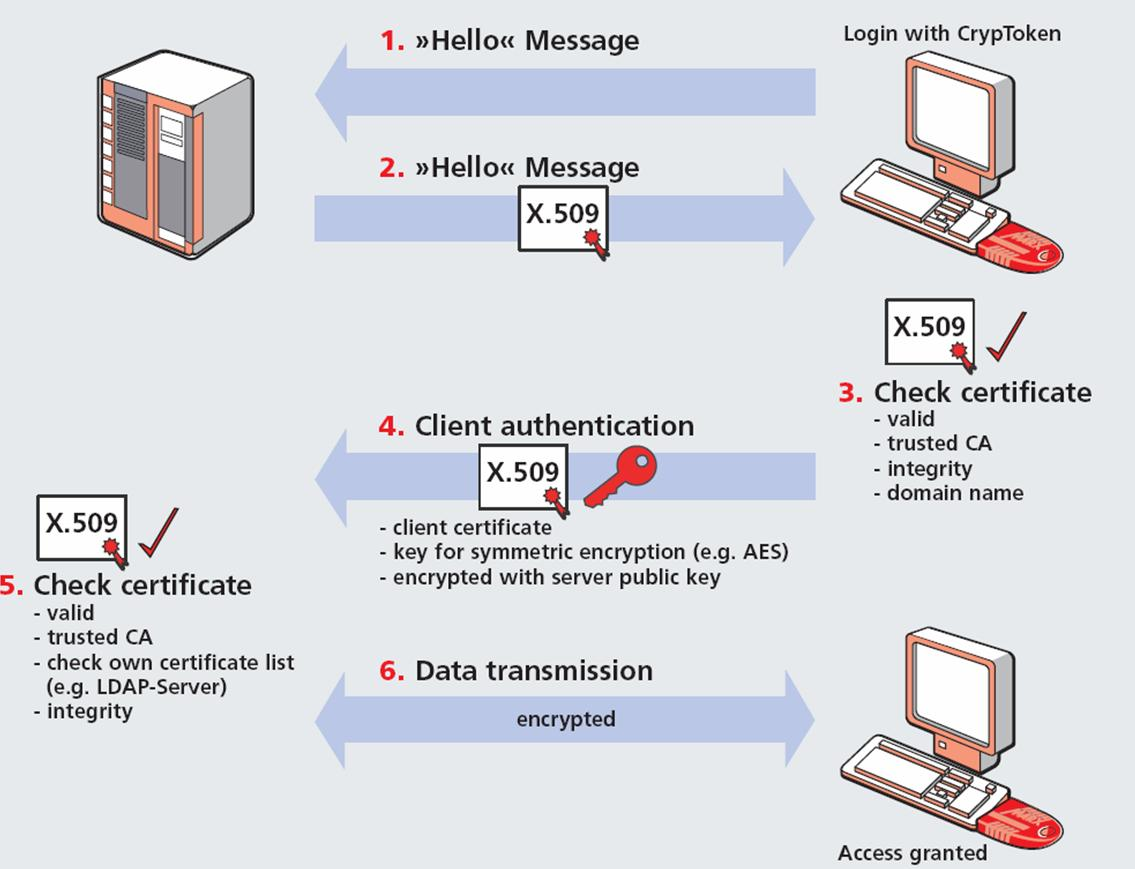
\includegraphics[width=\linewidth]{Images/TLS.jpg}
	\caption{Mutual TLS authentication}
	\label{fig:tls}
\end{figure}

TLS can be configured to authenticate both communicating parties. In the common HTTPS case, only the server presents a certificate: the client verifies that the certificate is valid, trusted, and associated with the requested domain name. In \textbf{mutual TLS authentication}, usually abbreviated as \textbf{mTLS}, the server also requests a certificate from the client. The client must then prove possession of the private key corresponding to that certificate (see figure \ref{fig:tls}).\\

The \texttt{CertificateRequest} message indicates that the server wants the client to authenticate with a certificate. The client answers by sending its own certificate and by proving that it owns the corresponding private key. The server then validates the client certificate before accepting the client as an authenticated endpoint.\\

When it is said that the server checks a certificate list, this should be understood as a simplified description of the server-side trust configuration. In practice, the server may verify that the client certificate satisfies several conditions:

\begin{itemize}
	\item the certificate is syntactically valid and has not expired;
	\item the certificate chain leads to a certification authority trusted by the server;
	\item the certificate has not been revoked, when revocation checking is used;
	\item the identity contained in the certificate corresponds to an accepted client, device, service, or organization;
	\item the authenticated identity is authorized to access the requested resource.
\end{itemize}

The server can be configured in different ways. In one approach, it trusts a specific certification authority used to issue client certificates. Any client certificate issued by that authority may then be accepted, possibly subject to additional authorization rules. In another approach, the server uses an explicit allowlist of accepted client certificates or certificate fingerprints. The first approach is more scalable, while the second is stricter but harder to manage when the number of clients grows.\\

This is the meaning of \textbf{controlled environments}. Mutual TLS is especially useful when the administrator can control or coordinate the creation, distribution, renewal, and revocation of client certificates. Typical examples include internal service-to-service communication, microservice platforms, administrative interfaces, enterprise systems, Internet-of-Things deployments, and business-to-business APIs. In such cases, the list of trusted client identities may effectively correspond to a list of internal services, managed devices, or business partners allowed to connect to the server.\\

Client-certificate authentication is different from authenticating a human user through a Web form or through an HTTP \texttt{Authorization} header. A client certificate primarily authenticates an endpoint or a certified identity at the TLS layer. That identity may correspond to a machine, a backend service, a device, an organization, or, less commonly, an individual user. The application may still need to map the authenticated certificate identity to application-level permissions, roles, or accounts before granting access to specific resources.\\

For this reason, mutual TLS provides \textbf{authentication} at the transport layer, but it does not automatically replace application-level \textbf{authorization}. After the TLS handshake has established that the client owns a trusted certificate, the application or gateway must still decide what that authenticated client is allowed to do.

\section{Relationship Between TLS Authentication and HTTP Authentication}

TLS authentication and HTTP authentication operate at different layers. TLS authenticates endpoints and protects the communication channel. HTTP authentication controls access to resources at the application protocol level. The two mechanisms can coexist.\\

For example, a browser may first establish a TLS-protected HTTPS connection and validate the server certificate. Only after that protected channel exists does the server return a \texttt{401 Unauthorized} response with a \texttt{WWW-Authenticate} challenge. The client then sends the corresponding \texttt{Authorization} header inside the already encrypted TLS channel.

\begin{lstlisting}
1. TLS authenticates the server and protects the channel.
2. HTTP authentication authenticates the user or client for a resource.
3. Authorization data is transmitted inside the TLS-protected channel.
\end{lstlisting}

This layering is important because HTTP authentication mechanisms such as Basic authentication do not by themselves protect credentials against network observation. When such credentials are sent over HTTPS, TLS provides the confidentiality that the HTTP authentication scheme does not provide on its own.

\section{Summary}

TLS is the transport security mechanism that makes HTTPS possible. It protects ordinary HTTP messages by carrying them inside a secure channel rather than by changing their application-level syntax. Its main guarantees are confidentiality, integrity, and endpoint authentication.\\

The TLS handshake uses PKI and X.509 certificates to authenticate endpoints, especially servers, and to establish cryptographic material. Asymmetric cryptography is used during the handshake, while symmetric encryption is used for efficient data transmission. Client and server negotiate the algorithms to be used, and TLS deployments must disable obsolete mechanisms in favor of robust cryptographic suites.\\

In the ordinary Web model, the client authenticates the server by validating its certificate chain, trust anchor, integrity, validity interval, and domain name. In mutual TLS configurations, the client can also authenticate to the server using a certificate. After the handshake, HTTP requests and responses are transmitted through the encrypted channel.\\

The security boundary of TLS is always the boundary between TLS endpoints. When a reverse proxy terminates TLS, it becomes part of the trusted path and may optionally establish another TLS session toward the origin server. Correctly identifying these endpoints is essential for understanding what HTTPS protects and where additional protection may be required.

\end{document}
